\chapter{Developing an Accurate GBC Detector}
%
\label{chap:gbcnet}
%
In this chapter, we systematically explore the potential of Deep Convolution Neural Network (CNN) models for accurately detecting Gallbladder Cancer (GBC) from Ultrasound (USG) images. As outlined in \cref{chap:intro}, USG is the predominant diagnostic modality for gallbladder (GB) diseases due to its affordability and accessibility. However, the analysis of USG images for GBC detection presents challenges such as low image quality, noise, and varying viewpoints resulting from the handheld nature of the sensor. To address these challenges, we introduce GBCNet and a curriculum tailored to enhance GBC detection performance from USG. We present a comprehensive discussion on GBCNet and the curriculum in this chapter.
\par The contents of this chapter was published as the following paper:
\par [1] \textit{Soumen Basu, Mayank Gupta, Pratyaksha Rana, Pankaj Gupta, and Chetan Arora. ``Surpassing the human accuracy: detecting gallbladder cancer from USG images with curriculum learning.'' In Proceedings of the IEEE/CVF Conference on Computer Vision and Pattern Recognition (CVPR), pp. 20886-20896, 2022}.

\section{Introduction}
%
Gallbladder cancer (GBC) is characterized by its aggressive nature, progressing rapidly if left untreated. Often, the disease advances silently, with malignancy extending into the neighboring liver and subsequently spreading to distant organs (called metastasis). Early diagnosis and resection are critical for improving the survival rate of \gbc. USG, on the other hand, stands out as the predominant diagnostic imaging modality for investigating patients with suspected gallbladder ailments \cite{klibanov2015ultrasound}, making it an excellent candidate modality for early detection of GBC. The advantages of USG include its affordability, accessibility, absence of ionizing radiation, and portability. Particularly in low-resource countries, the access to CT or MRI is limited due to high costs and their availability is also restricted to a few selected care centers. USG proves to be an invaluable diagnostic tool for early detection and intervention to GBC in such low-resource settings.

\par While identifying anomalies like stones or thickening of the GB wall during routine ultrasound (USG) is straightforward, precise characterization wall thickening remains challenging for even the most experienced radiologists \cite{gbc-lancet, gb-rads-paper, gupta2020imaging}. Although GBC typically presents with irregular wall thickening, early stages may exhibit smooth and symmetric thickening, which is similar to benign conditions \cite{gupta2020imaging}. As discussed earlier in \cref{sec:clinical}, traditional signs of benign thickening, such as echo-layering, can be present in malignant cases, complicating diagnosis. Moreover, various other medical conditions, including acute cholecystitis and hepatic, renal, and heart issues, can also cause gallbladder wall thickening, further complicating differentiation between benign and malignant causes. Frequently, USG is the only diagnostic imaging conducted for patients with suspected GB ailments. In cases where malignancy is not suspected, further testing is typically omitted, potentially allowing GBC to progress silently. Hence, there is an imperative need to develop effective characterization for GB malignancy from USG images. In pursuit of this objective, we turn to automated deep convolutional neural network (CNN)-based methods for gallbladder cancer (GBC) detection. Recent advancements in CNN-based machine learning (ML) models have yielded transformative progress in radiology and the diagnosis of various diseases, including breast cancer, lung cancer, pancreatic cancer, and melanoma \cite{ardila2019end, bejnordi2017diagnostic, chu2019application, codella2017deep, han2017breast}. However, the utilization of such models for GBC detection is notably absent. While prior efforts have focused on the segmentation and detection of GB abnormalities such as stones and polyps \cite{gbPolyp, gbPolyp2, gbAutomatic}, the specific detection of GBC from USG has not been attempted in prior literature.

\par However, there are significant challenges in using \cnn models for accurately detecting GBC from \usg image as discussed in \cref{sec:challenges}. %Unlike \mri or \ct, \usg images suffer from low imaging quality due to noise and other sensor artifacts such as acoustic shadow and echogenic textures as discussed in \Cref{sec:usg_artifact_issue}. The views are also not aligned due to the handheld nature of the sensor. 
Our study of state-of-the-art (\sota) CNN-based image classification techniques reveal that they often fail to learn the salient \gb region due to the presence of shadows, which may have similar visual traits of a \gb in \usg images (\cref{fig:teaser}). In addition to shadows, \gbc detection also gets biased towards learning from spurious textures due to noise and adjacent organ tissues rather than the shape or boundary of \gb wall, which impedes the accurate detection of GBC and results in poor GBC detection by off-the-shelf CNN models. Further, unlike normal and benign \gb regions, which have regular anatomy, malignant cases are much harder to detect precisely due to the absence of a clear \gb boundary or shape and the presence of a mass. %The lack of annotated dataset adds to the challenge of training the CNN models.

\begin{figure}[t]
    \centering
    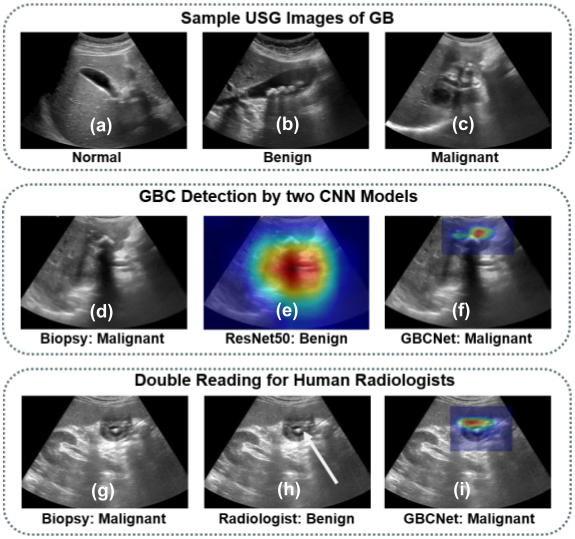
\includegraphics[width=0.6\textwidth]{figs/gbcnet/teaser.png}
    \caption[Depiction of issues with USG-based GBC detection]{(a), (b), and (c) Normal, benign, and malignant \gb sample in \usg images, respectively. While normal or benign \gb have regular anatomy, clear boundary is absent in malignant \gb. (d) A malignant (biopsy-proven) \gb sample. (e) Shadows having visual traits of a \gb leads to localization error in ResNet50. (f) \gbcnet tackles shadow artifacts well. (g) Another sample of malignant \gb. (h) The radiologist incorrectly diagnosed the \gb as benign based on the stone and wall thickening. (i) \gbcnet helps the radiologist to identify the salient region with liver infiltration by the \gb, a critical feature of \gbc, and correct the prediction.}
    \label{fig:teaser}
\end{figure}

\par In addressing this gap, we present the following significant contributions aimed at achieving highly accurate gallbladder cancer (GBC) detection from ultrasound (USG). Our primary goal is to ensure that our model exhibits a high recall (sensitivity) in detecting GBC. This emphasis on high recall is crucial as false negatives, where malignant cases are incorrectly predicted as non-malignant, can have severe consequences for the patients. On the other hand, the false positive prediction of malignancy can impose significant clinical, financial, and emotional burdens on the patients. It is thus essential to ensure that the model also shows high specificity (true negative rate).

%We propose GBCNet to tackle the challenges in our problem. GBCNet first extracts the regions of interest (\rois) by detecting the \gb (and not the cancer), and then uses a new multi-scale, second-order pooling architecture specializing in classifying \gbc. To effectively handle spurious textures, we propose a curriculum inspired by human visual acuity, which reduces the texture biases in GBCNet. Experimental results demonstrate that GBCNet significantly outperforms \sota \cnn models, as well as the expert radiologists. Our technical innovations are generic to other \usg image analysis tasks as well. Hence, as a validation, we also show the efficacy of GBCNet in detecting  breast cancer from \usg images. 
%Project page with source code, trained models, and data is available at \url{https://gbc-iitd.github.io/gbcnet.html}
\noindent \mypara{Contributions:}
\begin{enumerate}%[label=\textbf{(\arabic*)}]
	\item We focus on circumventing the challenges for automated detection of \gbc from \usg images and propose a deep neural network, GBCNet, for detecting \gbc from \usg images. GBCNet first extracts candidate regions of interest (\rois) by detecting the \gb (and not the cancer) from the \usg to mitigate the effects of shadows. Following the \roi detection, GBCNet employs a new  multi-scale, second-order pooling-based (MS-SoP) classifier on the \rois to classify gallbladder malignancy. MS-SoP encodes rich feature representations for malignancy detection. Experimental results demonstrate that GBCNet significantly outperforms multiple \sota \cnn models, as well as the expert radiologists. 
	%
	\item Even though GBCNet shows improvement in \gb malignancy detection over the \sota models, the spurious texture present in an \roi bias the classification unit towards generating false positives. To alleviate the issue, we propose a training curriculum inspired by human visual acuity \cite{kwon2016compensation, vogelsang2018VisualAcuity}. Visual acuity refers to the sharpness of visual stimuli. Studies suggest that an initial period of low visual acuity followed by high visual acuity helps the visual cortex in humans to formulate a better receptive field and emphasizes features such as shape or structure while identifying objects. 
	The proposed curriculum mitigates texture bias and helps GBCNet focus on shape features important for accurate \gbc detection from \usg images. % We validate the same in the context of \gbc detection from \usg images. %only, where we show in our experiment that our model after training with the proposed curriculum better focuses on GB boundaries.
	%
	\item A lack of publicly available \usg image datasets related to \gb malignancy adds to the difficulty of utilizing \cnn models for detecting \gbc. As discussed in \Cref{chap:data}, we have collected, annotated, and curated a \usg image dataset of 1255 abdominal \usg images. The dataset is referred as the Gallbladder Cancer Ultrasound (GBCU) dataset, and was publicly released with this work.
	%The dataset is available to the community.
	%post-acceptance of the paper after signing the necessary privacy agreement with our hospital. 	
\end{enumerate}


%
\section{Introduction}
%
According to GLOBOCAN 2018 \cite{bray2018global}, worldwide about 165,000 people die of \gbc annually. For most patients, \gbc is detected at an advanced stage, with a mean survival rate for patients with advanced \gbc of six months and a 5-year survival rate of 5\% \cite{randi2006gallbladder, gupta2021locally}. Detecting \gbc at an early stage could ameliorate the bleak survival rate. 

Lately, machine learning models based on convolutional neural network (\cnn) architectures have made transformational progress in radiology, and medical diagnosis for diseases such as breast cancer, lung cancer, pancreatic cancer, and melanoma \cite{ardila2019end, bejnordi2017diagnostic, chu2019application, codella2017deep, han2017breast}. However, their usage is conspicuously absent for the \gbc detection. Although there has been prior work involving segmentation and detection of the \gb abnormalities such as stones and polyps \cite{gbPolyp, gbPolyp2, gbAutomatic}, detection of \gbc is missing from the list. A search on Google Scholar with keywords ``artificial intelligence'' and ``gallbladder cancer'' returned 204 articles between 2015-2021. In these, we did not find any published article on deep learning-based \gbc detection from \usg images.

%\par According to GLOBOCAN 2018, GBC causes 165,087 deaths and 219,420 incidences every year worldwide \cite{armitage2014abeloff, bray2018global}. 
%%GBC is one of the leading causes of cancer-related deaths among Indian women \cite{randi2006gallbladder, bray2018global}. 
%The disease is prevalent in China, India, and Latin America. Canada, Australia, USA, and Europe also face a high incidence of GBC. 
%%\figref{fig:sec1-1} shows the detailed distribution of the incidence rate around the world.  
%GBC is detected at an advanced and metastasized stage for most patients, impeding curative resection and resulting in a dismal prognosis \cite{randi2006gallbladder, gupta2021locally}. 
%The overall mean survival rate for patients with advanced GBC is six months, with a 5-year survival rate of 5\%. 
%%In the USA, only about 1 in every 5 cases of GBC are identified in an early stage \cite{howlader2017seer}.
 
Early diagnosis and resection are critical for improving the survival rate of \gbc. Due to the non-ionizing radiation, low cost, portability, and accessibility, \usg is a popular diagnostic imaging modality. Although identifying anomalies such as stones or \gb wall thickening at routine \usg is easy, accurate characterization of the wall thickening is challenging \cite{gupta2020imaging, gb-rads-paper}. Often, \usg is the sole diagnostic imaging performed for patients with suspected \gb ailments. If malignancy is not suspected, no further testing is usually performed, and \gbc could silently advance. Therefore, it is imperative to develop and understand the characterization of \gb malignancy from \usg images.

There are significant challenges in using \cnn models for \usg image analysis. Unlike \mri or \ct, \usg images suffer from low imaging quality due to noise and other sensor artifacts. The views are also not aligned due to the handheld nature of the sensor. We observe that modern \cnn classifiers fail to localize the salient \gb region due to the presence of shadows which often have similar visual traits of a \gb in \usg images (\cref{fig:teaser}). Training object detectors for \gbc detection gets biased towards learning from spurious textures due to noise and adjacent organ tissues rather than the shape or boundary of \gb wall, which results in poor accuracy. Further, unlike normal and benign \gb regions, which have regular anatomy, malignant cases are much harder to detect due to the absence of a clear \gb boundary or shape and the presence of a mass.

\mypara{Contributions} 
%
The key contributions of this work are:
%\vspace{-0.5em}
\begin{enumerate}%[label=\textbf{(\arabic*)}]
%\itemsep-0.5em
	\item We focus on circumventing the challenges for automated detection of \gbc from \usg images and propose a deep neural network, GBCNet, for detecting \gbc from \usg images. GBCNet extracts candidate regions of interest (\rois) from the \usg to mitigate the effects of shadows and then uses a new  multi-scale, second-order pooling-based (MS-SoP) classifier on the \rois to classify gallbladder malignancy.
    %The first two stages of GBCNet are inspired by two-stage object detectors but focus only on detecting the \gb (and not cancer) and selecting a focused region of interest (\roi) to mitigate the effects of shadows. The third stage uses a new multi-scale, second-order pooling (MS-SoP) architecture to classify gallbladder malignancy.
	MS-SoP encodes rich feature representations for malignancy detection. 
	%
	\item Even though GBCNet shows improvement in \gb malignancy detection over multiple \sota models, the spurious texture present in an \roi bias the classification unit towards generating false positives. To alleviate the issue, we propose a training curriculum inspired by human visual acuity \cite{kwon2016compensation, vogelsang2018VisualAcuity}. Visual acuity refers to the sharpness of visual stimuli. %Studies suggest that an initial period of low visual acuity followed by high visual acuity helps the visual cortex in humans to formulate a better receptive field and emphasizes features such as shape or structure while identifying objects. 
	The proposed curriculum mitigates texture bias and helps GBCNet focus on shape features important for accurate \gbc detection from \usg images.% We validate the same in the context of \gbc detection from \usg images. %only, where we show in our experiment that our model after training with the proposed curriculum better focuses on GB boundaries.
	%
	\item A lack of publicly available \usg image datasets related to \gb malignancy adds to the difficulty of utilizing \cnn models for detecting \gbc. We have collected, annotated, and curated a \usg image dataset of 1255 abdominal \usg images collected from 218 patients. We refer this dataset as the Gallbladder Cancer Ultrasound (GBCU) dataset.
	%The dataset is available to the community.
	%post-acceptance of the paper after signing the necessary privacy agreement with our hospital. 	
\end{enumerate}

%

\section{Related Work}

\myfirstpara{Deep Learning for GB Abnormalities}
%
\usg imaging is an effective modality for diagnosing \gbc and related \gb afflictions \cite{yuan2018gbcManual}. 
%Recently, deep learning has been used as a diagnostic tool in medical imaging to great effect \cite{litjens2017dlmedical}. 
%Multiple studies have shown the application of these techniques on GB-related ailments, such as the detection of GB stones, biliary artesia, cholecystitis, and polyps. 
Lien \etal \cite{gbAutomatic} use a parameter-adaptive pulse-coupled neural network for \gb stone segmentation in \usg images. Pang \etal \cite{gbYolo} identify \gb and gallstones using a YOLOv3 model from \ct images. %Chen \etal \cite{gbPolyp} suggest an approach that segments the GB region followed by an AdaBoost classifier for diagnosing polyps. 
Jeong \etal \cite{gbPolyp2} uses an InceptionV3 model to classify neoplastic polyps from cropped samples of \gb \usg images. \gbc is a serious problem affecting a significant number of people. Despite the presence of numerous studies on using deep learning on other \gb-related afflictions, there is an absence of any work that applies deep learning to \gbc detection.

\mypara{Deep Learning for USG}
%
\cnn models have been widely applied in a plethora of \usg-based imaging tasks.
Mishra \etal proposed a fully convolutional neural network with deep attentional supervision on USG images for segmentation of blood vessel, liver lumen, and lesion \cite{mishra2018USSegmentation}. Deep learning-based segmentation models such as U-Net or Link-Net have been used to measure head circumference in fetal USG images \cite{budd2019FetalHC, sobhaninia2019FetalHC}. %VGG16-based architectures have been used for detecting the fetal scan plane \cite{baumgartner2017PlaneDetection}. 
Azizi \etal proposed a Deep Belief Network for detecting prostate cancer from USG images \cite{azizi2015ultrasound}. Li \etal modified Faster-RCNN for improving the detection of papillary thyroid cancer from USG \cite{li2018improved}. Deep learning has also been used in ovarian cancer \cite{zhang2019improved}, metastatic lymph node \cite{lee2018deep}, and breast cancer detection \cite{almajalid2018development, becker2018classification, cao2019BreastLesion, yap2018breast}. Zhu \etal recently proposed an attention-guided second-order sub-region pooling network for exploiting higher-order correlation to extract complex features from USG images \cite{zhu2020second}. A study by Ning \etal implemented a multi-scale higher-order pooling-based solution for breast lesion classification on USG images \cite{ning2020multi} .
%\cnn models have been widely applied in \usg imaging tasks, such as ovarian cancer detection \cite{zhang2019improved}, breast cancer region, mass and boundary detection \cite{bian2017boundary, cao2019BreastLesion, yap2018breast, ning2020multi, zhu2020second}, measuring head circumference in fetal \usg images \cite{sobhaninia2019FetalHC, budd2019FetalHC}. %, and other medical imaging and diagnostic applications. 

%\cite{mishra2018USSegmentation} proposed a fully convolutional neural network with deep attentional supervision on USG images for segmentation of blood vessel, liver lumen, and lesion. Deep learning-based segmentation models such as U-Net or Link-Net have been used to measure head circumference in fetal USG images \cite{sobhaninia2019FetalHC, budd2019FetalHC}. VGG16-based architectures have been used for detecting the fetal scan plane \cite{baumgartner2017PlaneDetection}. \cite{azizi2015ultrasound} proposed a Deep Belief Network for detecting prostate cancer from USG images. \cite{li2018improved} suggested modifications to Faster-RCNN for improving the detection of papillary thyroid cancer from USG. Deep learning has been used in ovarian cancer \cite{zhang2019improved}, metastatic lymph node \cite{lee2018deep}, and breast cancer detection \cite{cao2019BreastLesion, yap2018breast, almajalid2018development, becker2018classification}. \cite{zhu2020second} suggested an attention-guided second-order sub-region pooling network for exploiting higher-order correlation to extract complex features from USG images. A study by \cite{ning2020multi} proposes a multi-scale higher-order pooling-based solution for breast lesion classification on USG images. \cite{wang2020auto} used reinforcement learning to auto-assign weights to multimodal USG framework. 

\mypara{Curriculum Learning}
%
Curriculum learning has been applied to different medical imaging tasks. While Jesson \etal \cite{jesson2017cased} used a patch-based curriculum for lung nodule detection, Tang \etal \cite{tang2018attention} used disease severity level to identify thoracic diseases from chest radiographs. Oksuz \etal \cite{oksuz2019automatic} proposed image corruption-based curriculum to detect motion artifacts in cardiac \mri. 

\mypara{Texture Bias in Neural Networks}
%
Presence of mass and a thickened \gb wall are prominent indicators of \gb abnormality. However, typical \cnn-based architectures are biased towards textures rather than shape \cite{geirhos2018Texture}. This may lead GBCNet to focus on soft tissue textures such as liver rather than noticing cues based on the shape and wall of the \gb. 
%Therefore, a strategy is needed to reduce this texture bias of the network. 
Multiple works have attempted to reduce texture bias and improve the spatial understanding of a model. Geirhos \etal \cite{geirhos2018Texture} suggest style transfer to replace the original texture of images while Brendel \etal \cite{brendel2019BagOfFeatures} propose a method similar to a Bag of Features model to force spatial learning. 

\mypara{Visual Acuity in Learning Models}
%
Vogelsang \etal \cite{vogelsang2018VisualAcuity} suggest that a period of low visual acuity (blurred vision) followed by high visual acuity induces better spatial processing and also increases the receptive field in human vision. 
%Some recent works seem to follow the broad strategy and overcome the texture bias problem using blurring or similar other operations. 
Different from our visual acuity-inspired strategy of working with input space, Sinha \etal \cite{sinha2020curriculumBySmoothing} propose applying a Gaussian kernel on the output feature map of every layer of a network. The use of blurring before pooling seems to mitigate aliasing effects due to sub-sampling in the pooling layer rather than the use of visual acuity. Azad \etal \cite{azad2020textureDoG} have integrated a Difference of Gaussian (DoG) operation into their model. Similar to \cite{sinha2020curriculumBySmoothing}, they end up attenuating the high frequency in the feature maps corresponding to every layer rather than the input image, for which there is no obvious biological connection known. On the other hand, our proposed visual acuity-based curriculum works in the input space and has a solid neural basis \cite{vogelsang2018VisualAcuity}.


\begin{figure}[t]
	\centering
	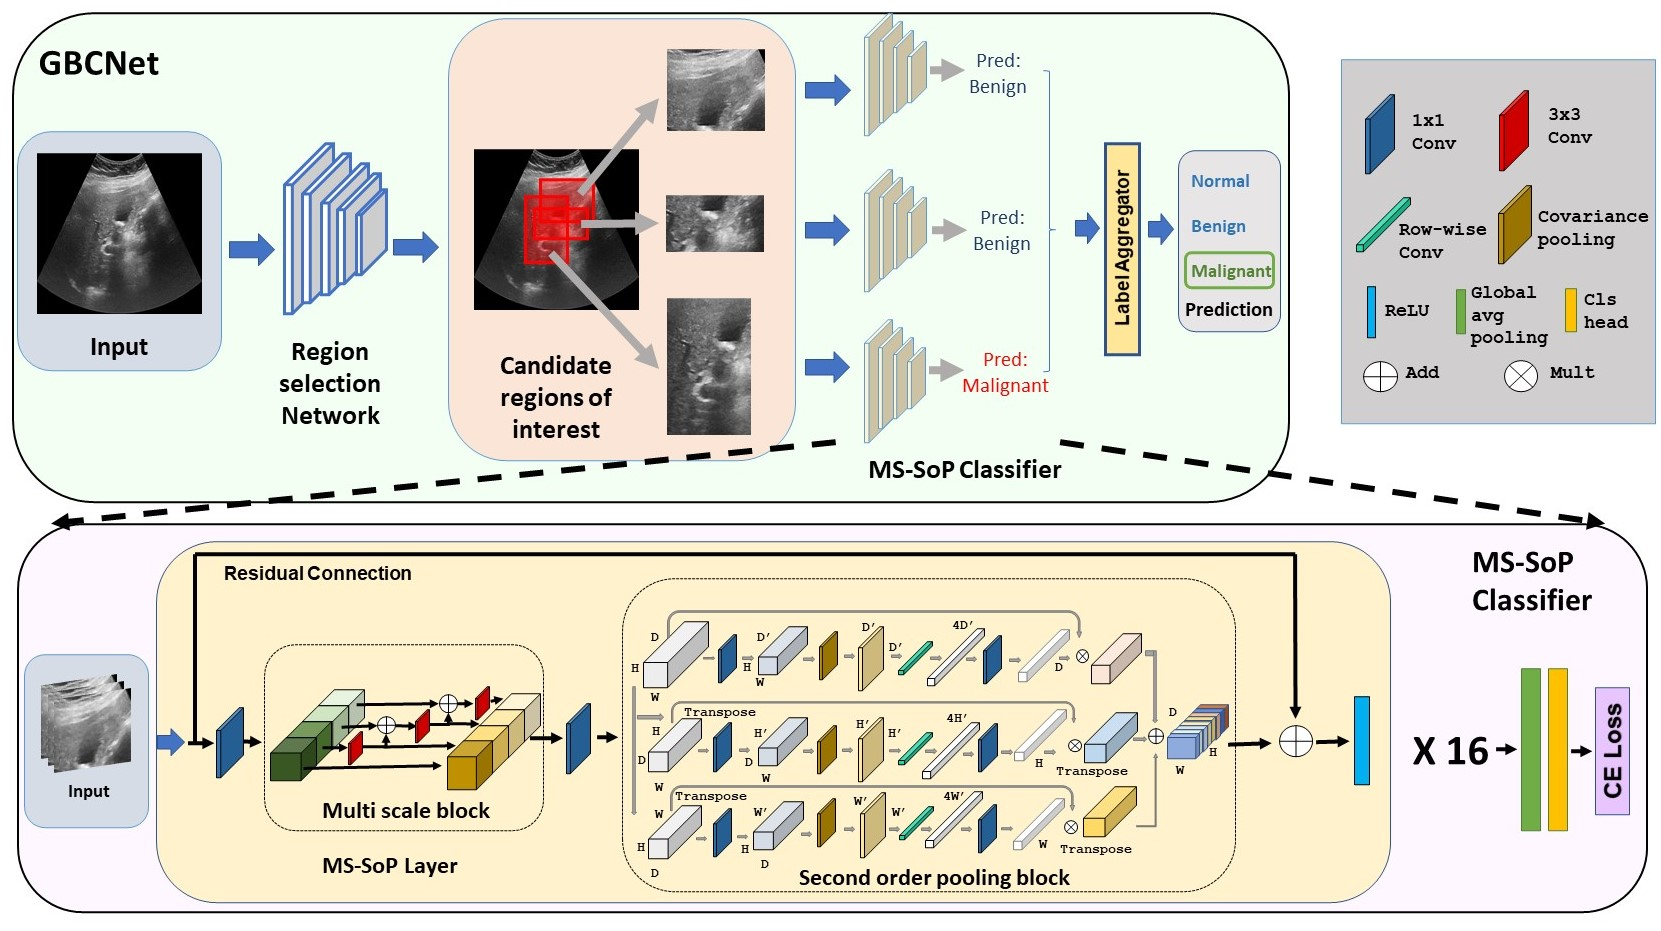
\includegraphics[width=\textwidth]{figs/gbcnet/arch-compact.jpg}
	\caption[Architecture of GBCNet]{Overview of the \gbcnet architecture. The region selection network localizes the candidate regions of interest and the multi-scale, second-order pooling-based (MS-SoP) classifier at the next stage predicts malignancy for each region. The predictions for each region is aggregated to get the final prediction on the whole image.}
	\label{fig-arch-overview}
\end{figure}


\section{Our Method}
%
\subsection{GBCNet: Model Architecture}
%
%Unlike CT or MRI, \usg images suffer from much higher noise levels and artifacts such as shadow due to \gb stones. 
The artifacts in \usg images often result in multiple spurious areas in a \usg image with very similar visual traits as the \gb region, leading to a disappointing performance by the baseline classifiers. 
%We have developed a CNN-based model, referred to as GBCNet, which can successfully detect \gbc, despite all the challenges described above. 
GBCNet selects candidate regions of interest (\rois) from the \usg to mitigate the influence of spurious artifacts like shadows and then uses a multi-scale, second-order pooling-based (MS-SoP) classifier on the \rois. \cref{fig-arch-overview} presents a conceptual diagram of the architecture. 
%We train a deep object detector to localize the \gb in the \usg images and generate the candidate ROIs to mitigate the influence of spurious artifacts. 
%The ROIs are cropped from the RGB images and passed to the MS-SoP classifier, to predict \gb malignancy.
At test time, the detector may predict multiple \rois overlapping with the \gb. Occasionally, the detection network may fail to localize the \rois. In this case, we pass the entire image to the classifier. The proposed MS-SoP classifier exploits a range of spatial scales 
%through multiple receptive fields during the feature encoding. In addition, the classifier utilizes 
and second-order statistics to generate rich features from \usg images to learn the characteristics of malignancy. We run the classifier for each candidate region during inference and aggregate the predicted labels to compute the prediction for the entire image. If any of the \rois is classified as malignant, the image as a whole is classified as malignant. If all the regions are predicted to be normal, the image is classified as normal. In all other cases, the image is predicted to be benign. 
%\par We observe that the above configuration of \gbCNet, though improving the detection of malignancy, still has a high false-positive rate. Our analysis shows that this is due to the texture bias of neural network models, which has been reported for the natural images as well \cite{geirhos2018Texture}. Inspired by human visual acuity, we propose a novel customized curriculum training regimen for training the classifier module of GBCNet. The proposed training process mitigates the texture bias and helps GBCNet reach the reported performance level. In the following subsections, we discuss different components of the GBCNet.

\mypara{Candidate \roi Selection}
%
We used deep object detection networks to localize the \gb region in a \usg image. The predicted bounding boxes serve as candidate regions of interest and mitigate the adverse effect of noise and artifacts from non-\gb regions during the classification. For training the \roi selection models, we use only two classes - background and the \gb region. In this stage, we only detect the \gb and do not classify them as malignant or non-malignant. In principle, it is possible to do both in a single stage, but we observed 
%that the candidate regions suggested by first stage region proposal network are often shifted from the \gb region, and classifying malignancy based upon them leads to poorer results. After the second stage the regions gets refined to a greater accuracy, and we observed 
that using a separate classifier on the focused \rois leads to better accuracy. We note that our findings regarding the superiority of using classification on focused regions, instead of over the entire image, are consistent with other recent works \cite{lancet_pancreas, cao2019BreastLesion, fan2020inf, sirinukunwattana2016locality, eccv2020_devil_in_classification}. Prior studies demonstrate that modern object detection architectures such as YOLO \cite{yolov4} or Faster-RCNN \cite{fasterrcnn} can detect breast lesions in \usg images  \cite{cao2019BreastLesion}. On the other hand, recently proposed anchor-free approaches, such as Reppoints \cite{reppoints}, and CentripetalNet \cite{centripetalnet} can detect unconventionally sized objects such as \gb. Hence, we experimented with all the above approaches for \roi selection in our framework. 

\mypara{MS-SoP Classifier}
%
Feature extraction in deep neural networks typically rely on first-order statistics, which performs unsatisfactorily in modalities like \usg. The presence of noise and artifacts along with ambiguous organ boundaries add to the complexities of detecting \gbc from \usg images. 
Modeling higher-order statistics has gained popularity in recent years due to its enhanced ability to capture complex features and non-linearity in deep neural networks \cite{gao2019global, li2017second, zoumpourlis2017non}. %The presence of noise and artifacts along with ambiguous organ boundaries add to the complexities of detecting \gbc from ultrasound images. 
Ning \etal \cite{ning2020multi} recently used higher-order feature fusion for classifying breast lesions. They have used RGB image patches of three fixed scales at the input layer. We take the idea further and develop a novel multi-scale, second-order pooling (MS-SoP) layer to encode rich features suitable for malignant \gb detection. In contrast to \cite{ning2020multi}, we exploit feature maps of multiple scales in all the intermediate layers to learn a rich representation. The proposed MS-SoP layers can be conveniently plugged into any \cnn backbone.
%Further, instead of using the features at different resolutions, we use the multiple receptive fields to capture features at different scales. 
The MS-SoP classifier contains $16$ MS-SoP layers as the backbone, followed by global average pooling and a fully connected classification head. 
Each block uses multiple scales and second-order pooling to encode robust feature representation. %The 1$\times$1 convolutions resize the feature depth for computational efficiency. 
The MS-SoP classifier takes input of size $224\times224\times3$. As input \usg images are grayscale, we copy the resized image to all three channels. Using a first layer that directly takes as input the grayscale was possible in principle but would have denied us the opportunity to use pre-trained backbones. Consistent with the ones reported in the literature \cite{alzubaidi2020transferlearning, cheng2017transfer}, we observe that cross-domain fine-tuning of a pre-trained classifier gives better accuracy than training from scratch. 
We use the Categorical Cross-Entropy loss to train the classifier. 

%We have used a $7\times 7$ convolution layer and $16$ multi-scale, second-order pooling-based convolutional layers as feature extraction backbone of the classification network. The feature extraction backbone is followed by global average pooling, and a fully connected layer completes the classifier network. \cref{fig:gbc_block} presents a pictorial overview of the classifier, highlighting the feature extraction block. Each block uses multiple scales and second-order pooling to encode robust feature representation. The 1$\times$1 convolutions resize the feature map depth for computational efficiency. %Our designed classifier network contains 26.9M parameters. 
%The final softmax layer outputs probability for three classes representing normal, benign, and malignant \gb. The classifier takes input of size $224 \times 224 \times 3$. We crop the candidate ROIs from the input image as predicted by the region selection network and resize them to feed the classifier. As input \usg images are grayscale, we copy the resized image to all three channels. Using a first layer that directly takes as input the grayscale was possible in principle but would have denied us the opportunity to use pre-trained backbones. Consistent with the ones reported in the literature \cite{alzubaidi2020transferlearning, cheng2017transfer}, we observe that cross-domain fine-tuning of a pre-trained classifier gives better accuracy than training from scratch. We used the standard Categorical Cross-Entropy loss to train the classifier unit. 


\myfirstpara{Multi-Scale Block}
%
Abdominal organs can appear in significantly different sizes in a \usg image based on the insonation angle or the pressure on the transducer. Perceiving information across multiple scales is thus necessary for accurate \gbc detection. Recently, Gao \etal \cite{res2net} have replaced the standard convolution block in the bottleneck layer with group convolution to add a multi-scale capability to the ResNet architecture. Inspired by \cite{res2net}, we used a hierarchy of convolution kernels on slices of feature volumes in the intermediate layers to capture multi-scale information through a combination of different receptive fields. We split a feature map volume, $\mathcal{X} \!\in\!\mathbb{R}^{H\!\times\! W \!\times\! D}$ ($H, W ~\text{and}~D$ are the height, width, and the number of channels, respectively), depth-wise into 4 slices, $\mathcal{X}_1,\mathcal{X}_2,\mathcal{X}_3$, and $\mathcal{X}_4$, where $\mathcal{X}_i \!\in\! \mathbb{R}^{H\!\times\! W\!\times\! D/4}$. Each $\mathcal{X}_i$ will generate an output split $\mathcal{Y}_i$. The final output, $\mathcal{Y}$, is obtained by concatenating the splits. Suppose $\mathcal{C}_j$ are $3\!\times\!3$ convolution kernels and $\oast$ denotes the convolution. We get each $\mathcal{Y}_i$ as follows:
\linebreak
\begin{minipage}{.4\linewidth}
\vspace{-1em}
\begin{align}
    \mathcal{Y}_1 &= \mathcal{X}_1 \\
    \mathcal{Y}_2 &= \mathcal{C}_1 \oast \mathcal{X}_2
\end{align}
\end{minipage}
\begin{minipage}{.6\linewidth}
\vspace{-1em}
\begin{align}
    \mathcal{Y}_3 &= \mathcal{C}_2 \oast (\mathcal{X}_3 \!+\! \mathcal{Y}_2) \\
    \mathcal{Y}_4 &= \mathcal{C}_3 \oast (\mathcal{X}_4 \!+\! \mathcal{Y}_3)
\end{align}
\end{minipage}

\mypara{Second-order Pooling Block}
%
Traditional average or max-pooling use first-order statistics and thus cannot capture the higher-order statistical relation between features. Inspired by the recent success of higher-order statistics in breast lesion \usg \cite{ning2020multi, zhu2020second}, we employ the second-order pooling (SoP) mechanism to exploit the second-order statistical dependency between the multi-scale features.  

For computational efficiency, we reduce the number of channels of a feature volume, $\mathcal{X} \!\in\! \mathbb{R}^{H \!\times\! W \!\times\! D}$, to $D'~(D'\!<\!D)$, using $1\!\times\!1$ convolutions. $\mathcal{X}$ is then reshaped to a matrix $\vb{X} \!\in\! \mathbb{R}^{D'\!\times\! N}$, where $N\!=\!H\!\times\! W$. We compute the covariance of $\vb{X}$ as, $\vb{C}_{D'\!\times\!D'} \!=\! (\vb{X\!-\!\bar{X}})\vb{(X\!-\!\bar{X})^T}$, which is then reshaped to a tensor of size $1 \!\times\! D' \!\times\! D'$ and passed through a convolution layer with $4D'$ kernels of size $1 \!\times\! D'$ each. We resize the resulting $1\!\times\! 1 \!\times\! 4D'$ tensor to a $1\!\times\! 1 \!\times\! D$ tensor, $\vb{w_d}$, by $1\!\times\! 1$ convolutions. $\vb{w_d}$ represents the weight for each channel. These weights are then channel-wise multiplied with $\mathcal{X}$, to obtain the weighted feature map $\vb{Z_d}$. To repeat similar processes for the height and width, we transpose $\mathcal{X}$ from to a $D \!\times\! W \!\times\! H$ tensor, say $\mathcal{X}_h$ and to a $H \!\times\! D \!\times\! W$ tensor, say $\mathcal{X}_w$. In terms of index notation, $\mathcal{X}_h[k,j,i] \!=\! \mathcal{X}[i,j,k]$ and $\mathcal{X}_w[i,k,j] \!=\! \mathcal{X}[i,j,k]$, where $i\!=\!\{1,2,\ldots H\}, ~j\!=\!\{1,2,\ldots W\},$ and $k\!=\!\{1,2,\ldots D\}$. Similar to calculating $\vb{w_h}$ from $\mathcal{X}$, we find $\vb{w_h}\!\in\! \mathbb{R}^{1\!\times\!1\!\times\!H}$ from $\mathcal{X}_h$, and $\vb{w_w}\!\in\! \mathbb{R}^{1\!\times\!1\!\times\!W}$ from $\mathcal{X}_w$. We also calculate $\vb{Z_h}$ and $\vb{Z_w}$ by multiplying $\vb{w_h}$ and $\vb{w_w}$ channel-wise to $\mathcal{X}_h$ and $\mathcal{X}_w$. Then, we transpose $\vb{Z_h}$ and $\vb{Z_w}$ to tensors of size $H\!\times\! W \!\times\! D$, say $\vb{Z_h}^T$ and $\vb{Z_w}^T$, respectively, where $\vb{Z_h}^T[i,j,k] = \vb{Z_h}[k,j,i]$ and $\vb{Z_w}^T[i,j,k] = \vb{Z_w}[i,k,j]$. Finally, we obtain the output feature tensor, $\vb{Z} \!\in\! \mathbb{R}^{H\!\times\! W \!\times\! D}$ by adding $\vb{Z_d}, \vb{Z_h}^T,$ and $\vb{Z_w}^T$. 
\vspace{-0.5em}
\begin{align}
    \vb{Z_d}[i,j,k] &= \vb{w_d}[k] ~~ \mathcal{X}[i,j,k] \\
    \vb{Z_h}[k,j,i] &= \vb{w_h}[i] ~~ \mathcal{X}_h[k,j,i]  \\
    \vb{Z_w}[i,k,j] &= \vb{w_w}[j] ~~ \mathcal{X}_w[i,k,j]  \\
    \vb{Z}[i,j,k] &= \vb{Z_d}[i,j,k] + \vb{Z_h}^T[i,j,k] + \vb{Z_w}^T[i,j,k]
\end{align}
\vspace{-1em}
% The input feature volume, $\mathcal{X} \!\in\! \mathbb{R}^{H \!\times\! W \!\times\! D}$, where $H, W, \text{and}~D$ are the spatial height, width, and the number of channels. We reduce the number of channels to $D'~(D'<D)$, using $1\!\times\! 1$ convolutions to reduce computational cost. Thus, the feature tensor becomes $\mathcal{X} \!\in\! \mathbb{R}^{H \!\times\! W \!\times\! D'}$. Now, we reshape the feature tensor, $\mathcal{X}$, to a matrix $\vb{X} \!\in\! \mathbb{R}^{D'\!\times\! N}$, where $N=H\!\times\! W$. Adapting from \cite{li2017second}, we compute the sample covariance, $\vb{C} \!\in\! \mathbb{R}^{D' \!\times\! D'}$, of the feature matrix $\vb{X}$ (consisting of $N$ samples, each of dimension $D'$), as 
% \begin{align}
%     % c_{ij} &= \frac{1}{N-1} \sum\limits_{i=1}^N{(\vb{x_i} - \vb{\mu})(\vb{x_i}-\vb{\mu})^T}
%     \vb{C} = \vb{X}\vb{J}\vb{X^T}~,~~ \vb{J} = \frac{1}{N} \big[\vb{I_N} - \frac{1}{N} \vb{11^T} \big]
% \end{align}
% where $\vb{I_N}$ is an $N \!\times\! N$ identity matrix, $\vb{1} = [1,\ldots,1]^T$ is a $N$-dimension vector with all elements being one, and $T$ is the matrix transpose. 

% The $D'\!\times\! D'$ sized covariance matrix is then reshaped to a 3D tensor of size $1 \!\times\! D' \!\times\! D'$ and passed through a convolution layer with $4D'$ kernels of size $1 \!\times\! D'$ each. In other words, the convolution layer has $D'$ in-channels and $4D'$ out-channels. The resulting $1\!\times\! 1 \!\times\! 4D'$ tensor is resized to $1\!\times\! 1 \!\times\! D$ by $1\!\times\! 1$ convolution. This $1\!\times\! 1 \!\times\! D$ tensor, say $\vb{w_d}$, represents the weight for each channel/feature-map. These weights are then channel-wise multiplied with the original feature map, $\mathcal{X}$, to obtain the weighted feature map $\vb{Z_d}$, which is a $H \!\times\! W \!\times\! D$ tensor. 

% We repeat a similar process for the height and width as well. For this we transpose the feature map $\mathcal{X}$ from $H \!\times\! W \!\times\! D$ to a $D \!\times\! W \!\times\! H$ tensor, say $\mathcal{X}_h$ and to a $H \!\times\! D \!\times\! W$ tensor, say $\mathcal{X}_w$. We use the indices $i,j,$ and $k$ to express the 3-dimensional tensors where $i=\{1,2,\ldots H\}, j=\{1,2,\ldots W\},$ and $k=\{1,2,\ldots D\}$. Using the index notation, $\mathcal{X}_h[k,j,i] = \mathcal{X}[i,j,k]$ and $\mathcal{X}_w[i,k,j] = \mathcal{X}[i,j,k]$.
% The process mentioned above for the dimension D of $\mathcal{X}$ is similarly followed for dimension H of $\mathcal{X}_h$, to obtain the per channel/feature-map weights $\vb{w_h} \!\in\! \mathbb{R}^{1\!\times\! 1 \!\times\! H}$, and multiply them to $\mathcal{X}_h$ to obtain $\vb{Z_h} \!\in\! \mathbb{R}^{D\!\times\! W \!\times\! H}$. The same process is repeated for dimension W of $\mathcal{X}_w$ to get $\vb{w_w} \!\in\! \mathbb{R}^{1\!\times\! 1 \!\times\! W}$, and $\vb{Z_w} \!\in\! \mathbb{R}^{H\!\times\! D \!\times\! W}$. 
% Then, we transpose $\vb{Z_h}$ and $\vb{Z_w}$ to tensors of size $H\!\times\! W \!\times\! D$, say $\vb{Z_h}^T$ and $\vb{Z_w}^T$, respectively, where $\vb{Z_h}^T[i,j,k] = \vb{Z_h}[k,j,i]$ and $\vb{Z_w}^T[i,j,k] = \vb{Z_w}[i,k,j]$. Finally, we obtain the output feature tensor, $\vb{Z} \in \mathbb{R}^{H\!\times\! W \!\times\! D}$ by adding $\vb{Z_d}, \vb{Z_h}^T,$ and $\vb{Z_w}^T$. 
% \begin{align}
%     \vb{Z_d}[i,j,k] &= \vb{w_d}[k] ~~ \mathcal{X}[i,j,k] \\
%     \vb{Z_h}[k,j,i] &= \vb{w_h}[i] ~~ \mathcal{X}_h[k,j,i]  \\
%     \vb{Z_w}[i,k,j] &= \vb{w_w}[j] ~~ \mathcal{X}_w[i,k,j]  \\
%     \vb{Z}[i,j,k] &= \vb{Z_d}[i,j,k] + \vb{Z_h}^T[i,j,k] + \vb{Z_w}^T[i,j,k]
% \end{align}

\begin{figure}[t]
    \centering
    \begin{subfigure}[b]{0.3\linewidth}
		\centering
		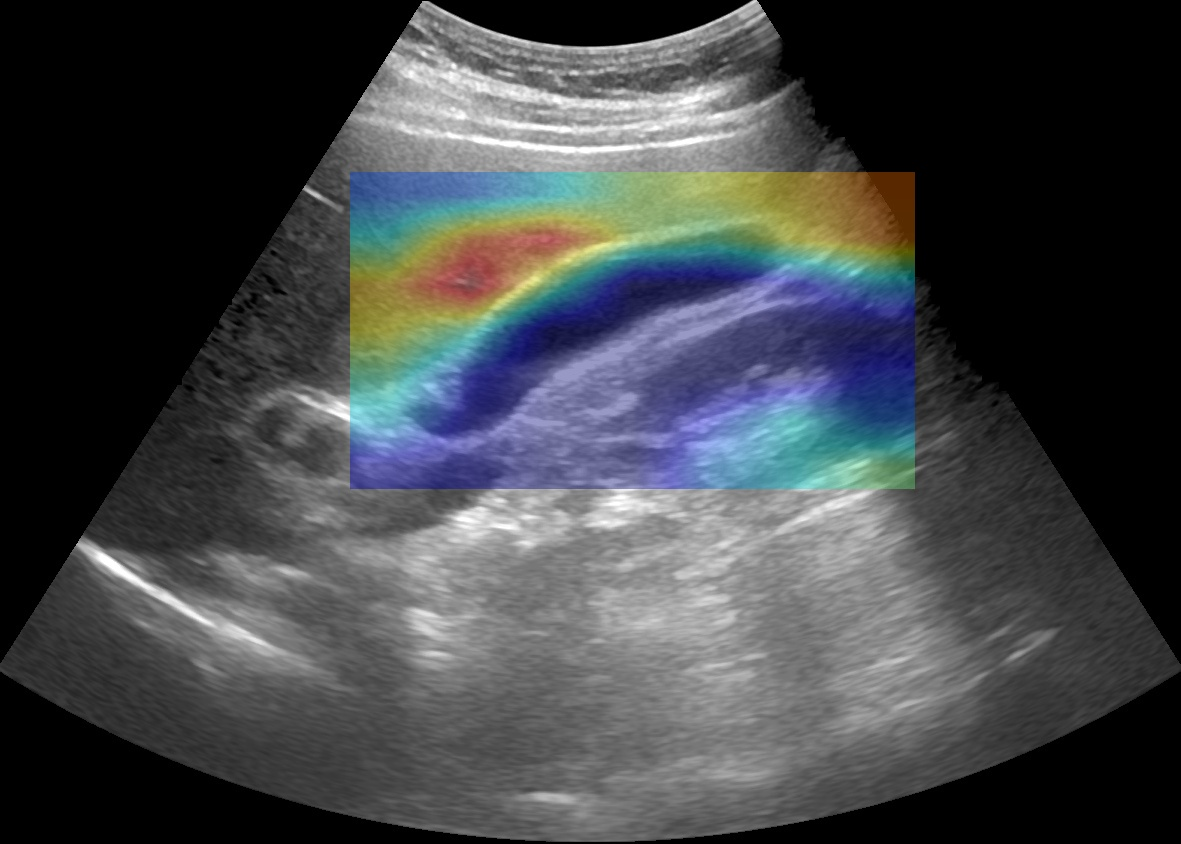
\includegraphics[width=\linewidth,height=8em]{figs/gbcnet/texture-1.jpg}
		\caption{}
		%\label{fig:multi-scale}
	\end{subfigure}
    \begin{subfigure}[b]{0.3\linewidth}
		\centering
		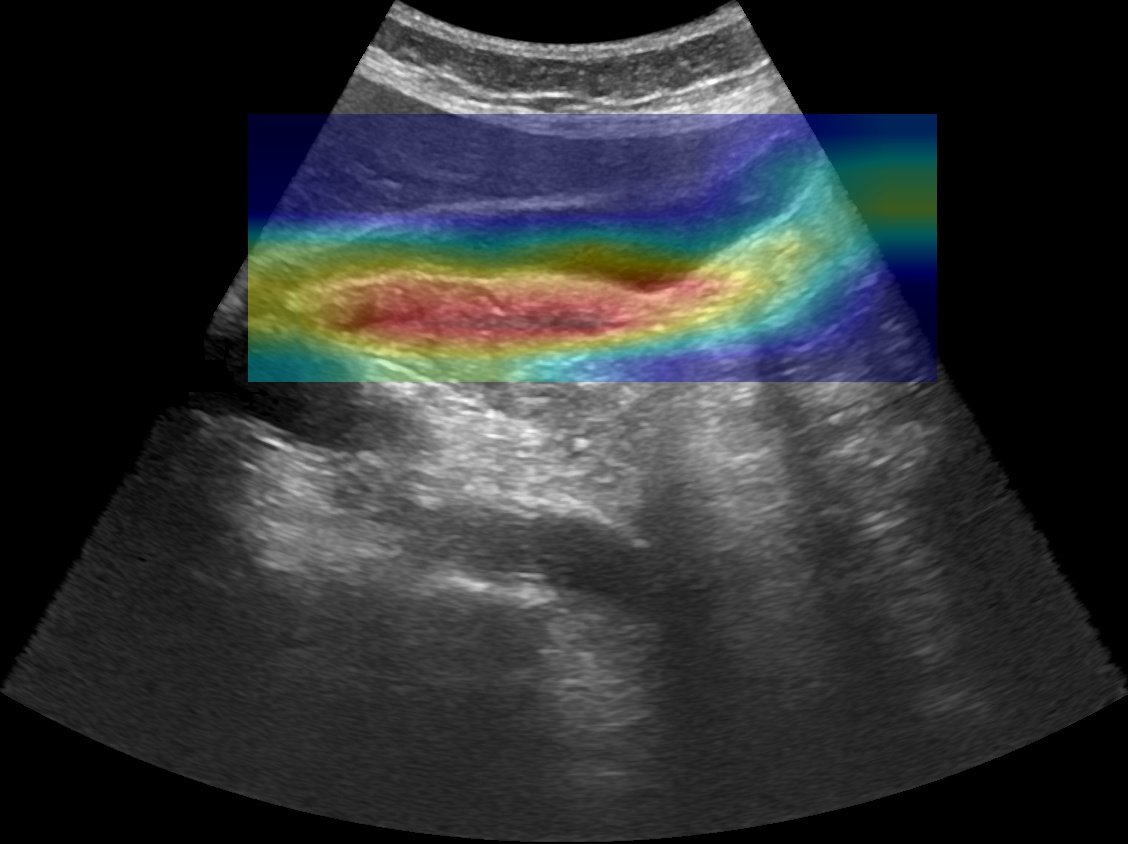
\includegraphics[width=\linewidth,height=8em]{figs/gbcnet/texture-2.jpg}
		\caption{}
		%\label{fig:multi-scale}
	\end{subfigure}
	\begin{subfigure}[b]{0.3\linewidth}
		\centering
		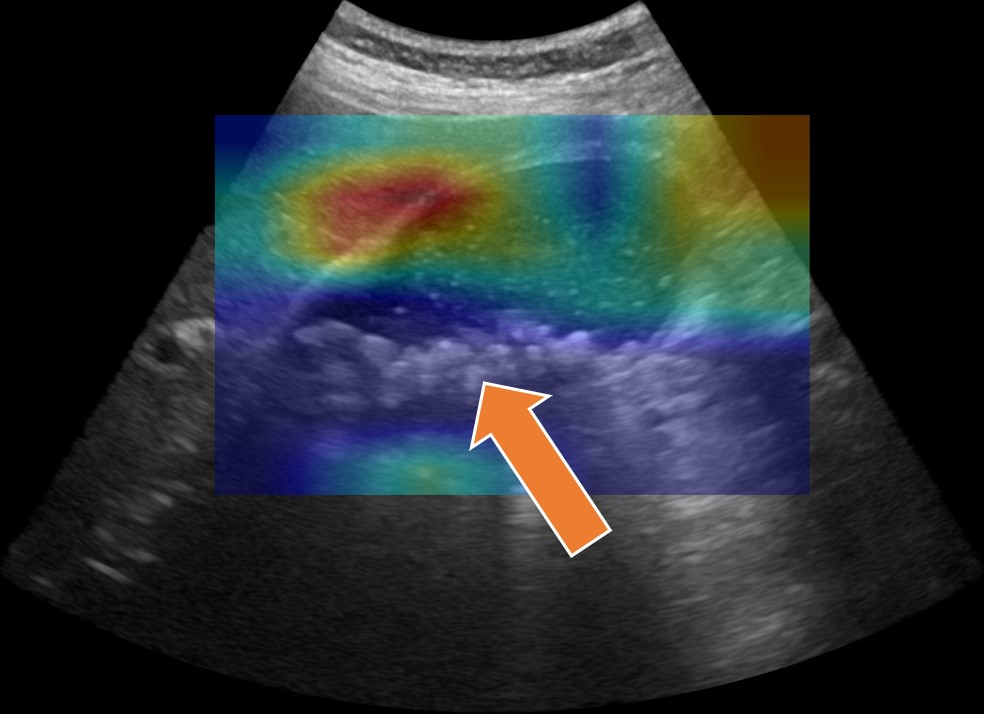
\includegraphics[width=\linewidth,height=8em]{figs/gbcnet/texture-3.jpg}
		\caption{}
		%\label{fig:multi-scale}
	\end{subfigure}
    \caption[Visualization of texture bias]{Grad-CAM visual of GBCNet trained without curriculum showing how the model tends to get biased due to the presence of textures due to noise or organ tissue. GBCNet focuses on - (a) adjacent liver tissues than the normal \gb, (b) the echogenic region below the \gb, and (c) liver textures instead of the stones (highlighted using the arrow).}
    \label{fig:texture_bias_sample}
\end{figure}
%
\begin{figure}[t]
	\centering
	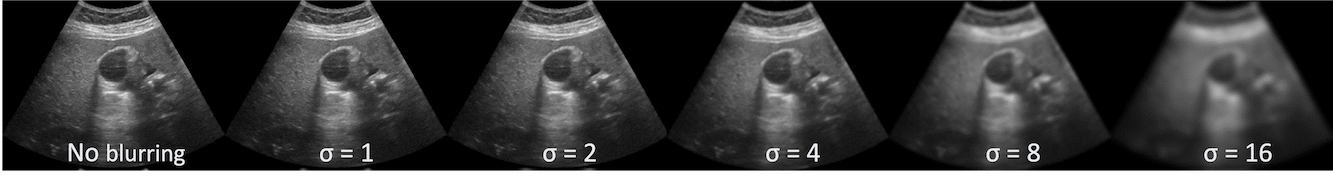
\includegraphics[width=0.95\linewidth]{figs/blur_sample_1.png}
	\caption[Gaussian blurring of USG data samples]{We simulate visual acuity through the Gaussian blur. Increasing $\sigma$ in a Gaussian filter decreases the visual acuity. Notice in the figure that, the effect of textures reduce as the visual acuity decreases and \gb shape and structure become more pronounced.}
	\label{fig:vis_acuity_sample}
\end{figure}

%% Curriculum
\subsection{Visual Acuity Inspired Curriculum}
%
We found that the textures having visual characteristics of soft tissue can adversely affect the performance of GBCNet (\cref{fig:texture_bias_sample}). We propose a curriculum to mitigate the texture bias and improve the classification. We observed that while the MS-SoP classifier is affected by texture bias, the region selection network still maintains a very high recall (\cref{tbl:perf_region}). Hence, we used the curriculum training only on the classifier and not on the region selection network.

\mypara{Visual Acuity in Humans}
%
Visual Acuity (VA) refers to the clarity and sharpness of human vision. Due to the immaturity of the retina and visual cortex, newborn children have very low VA \cite{courage1990visual}. The VA improves with the maturation of the retina and visual cortex. However, for children with congenital cataracts, the cortex matures despite the lenticular opacity. Such children begin their visual activity with higher initial VA. Evidence shows that children with high initial VA suffer to facilitate spatial analysis over expansive areas \cite{vogelsang2018VisualAcuity}.  Low VA renders blurry images that do not contain enough local information for the visual cortex to identify patterns. As a result, the visual cortex tries to increase the receptive field to facilitate spatial analysis over expansive areas and learn global features \cite{kwon2016compensation, smith2009smile}. 

\begin{algorithm}[t]
\small  
	\caption{Proposed Visual Acuity-based Curriculum}
	\label{va_algo}
	\SetAlgoLined
	\KwIn{$D^{\text{train}}$, Dataset of regions cropped from the original USG images.}
	\KwOut{Optimized model parameters $W^*$}
	Initialize $\sigma = \sigma_0$ \;
	%Set warm-up size to be $k'$ \;
	Initialize model parameters to $W$ \;
	
	\For {epoch=$\{1 \ldots, N\}$}{
		\eIf{$\sigma > 0$}{
		    $Z = \phi$ \;
    		\For {$x \in D^{\text{train}}$} {
    			$Z = Z \cup \{x \oast G(\sigma)\}$ \;
    		}
		    train($W, Z$)\;
		}
		{
		    train($W, D^{\text{train}}$) \;
		}
		\If{(epoch $> k'$) and (epoch$\%k == 0$)}{
			$\sigma = \lfloor \sigma/2 \rfloor$ \; 
		}
	}
\end{algorithm}


\mypara{Gaussian Blurring to Simulate Visual Acuity}
%
Gaussian filters are low-pass filters to cloak the high-frequency components of an input. A standard deviation $\sigma$ parameterizes the Gaussian filters. Increasing the $\sigma$ generates a higher amount of blur and low VA when convolved with an image. \cref{fig:vis_acuity_sample} shows how we can decrease the VA by increasing the $\sigma$ of a Gaussian filter. In our experiments, we have varied $\sigma$ from $1$ to $16$ to generate different levels of VA. 

\mypara{Proposed Curriculum}
%
While \cite{vogelsang2018VisualAcuity} demonstrates the improvement in receptive fields by gradually improving the sharpness of images during training, we take this observation further and show that the strategy of training on progressively higher resolution images also reduces the texture bias of a classification model. We propose a visual acuity-based training curriculum (\cref{va_algo}) that starts training the network with blurry and low-resolution \usg images and progressively increase the sharpness of training samples. The initial blurring allows the model to use an extended receptive field and focus on learning the global features such as the shape of the \gb while ignoring any noise or irrelevant textures. In the later phases, the sharp images allow the model to focus on the relevant local features in a controlled manner to make more accurate predictions. 


%\section{Dataset Collection and Curation}

\myfirstpara{Data Collection}
%
We acquired data samples from patients referred to PGIMER, Chandigarh (a tertiary care referral hospital in Northern India) for abdominal ultrasound examinations of suspected \gb pathologies. The study was approved by the Ethics Committee of PGIMER. We obtained informed written consent from the patients at the time of recruitment, and protect their privacy by fully anonymizing the data. Minimum 10 grayscale B-mode static images, including both sagittal and axial sections, were recorded by radiologists for each patient using a Logiq S8 machine. We excluded color Doppler, spectral Doppler, annotations, and measurements. Supplementary A %\ref{supp:data_collection} 
contains more details of the data acquisition process.

\mypara{Labeling and ROI Annotation}
%
Each image is labeled as one of the three classes - normal, benign, or malignant. The ground-truth labels were biopsy-proven to assert the correctness. Additionally, in each image, expert radiologists have drawn an axis-aligned bounding box spanning the entire \gb and adjacent liver parenchyma to annotate the \roi. 

\mypara{Dataset Statistics}
%
We have annotated 1255 abdominal \usg images collected from 218 patients from the acquired image corpus. Overall, we have 432 normal, 558 benign, and 265 malignant images. Of the 218 patients, 71, 100, and 47 were from the normal, benign, and malignant classes, respectively. The width of the images was between 801 and 1556 pixels, and the height was between 564 and 947 pixels due to the cropping of patient-related information. 

\mypara{Dataset Splits}
%
The sizes of the training and testing sets are 1133 and 122, respectively. To ensure generalization to unseen patients, all images of any particular patient were either in the train or the test split. The number of normal, benign, and malignant samples in the train and test set is 401, 509, 223, and 31, 49, and 42, respectively. Additionally, we report the 10-fold cross-validation metrics on the entire dataset for key experiments to assess generalization. All images of any particular patient appeared either in the training or the validation split during the cross-validation. 

%results table, pasted here for formatting reasons
%% Implementation

\section{Implementation Details}
 \begin{table}[t]
\centering
\scriptsize
%\setlength{\tabcolsep}{4pt}
    \resizebox{ \linewidth}{!}{%
        \begin{tabular}{p{0.1\linewidth}p{0.42\linewidth}p{0.06\linewidth}p{0.2\linewidth}p{0.05\linewidth}p{0.06\linewidth}}
        \toprule[1.5pt]
        \textbf{Model} & \textbf{Description} & \textbf{Input Size} & \textbf{Optimizer} & \textbf{Batch size} & \textbf{Epochs/ Steps}
        \\ \midrule[0.75pt]
        YOLOv4 \cite{yolov4} & CSPDarknet53 backbone, PANet neck, anchor-based YOLO head. Total 162-layers. Backbone was frozen for first 800 step. Entire network was trainable thereafter. Single stage, anchor-based  & $608\times608\times3$ & SGD LR = 0.0001 momentum = 0.95 weight decay = 0.0005 & 64 & 3000 steps \\ \hline
        Reppoints \cite{reppoints} & Resnet-101 backbone, Group Normalization neck, and a reppoints head. Backbone was frozen for first 30 epochs, and entire network was trainable thereafter. Two-stage, anchor-free & $800 \times 1333 \times 3$ & SGD LR = 0.001 momentum = 0.9 weight decay = 0.0001 & 4 & 50 epochs \\ \hline
        Centripetal-Net \cite{centripetalnet} & HourglassNet-104 backbone. Enitre network was trainable. Anchor-free & $511 \times 511 \times 3$ & Adam LR = 0.0005 & 4 & 50 epochs \\ \hline
        ResNet \cite{resnet} & Resnet-50 used. All layers were trainable. LR decays by 10\% after every 5 epochs through a step LR scheduler. & $224\times224\times3$ & SGD LR = 0.005 momentum = 0.9 weight decay = 0.0005 & 16 & 100 epochs \\ \hline
        VGG \cite{vgg} & VGG-16 is used. All layers were trainable. LR decays by 10\% after every 5 epochs through a step LR scheduler. & $224\times224\times3$ & SGD LR = 0.005 momentum = 0.9 weight decay = 0.0005 & 16 & 100 epochs \\ \hline
        Inception \cite{inception} & Inception-V3 used. All layers were trainable. LR decays by 10\% after every 5 epochs through a step LR scheduler. & $299\times299\times3$ & SGD LR = 0.005 momentum = 0.9 weight decay = 0.0005 & 16 & 100 epochs \\ \hline
        RetinaNet \cite{retinanet} & Resnet-18-FPN used as backbone. All layers were trainable. & $512\times512\times3$ & Adam LR = 0.0001 & 8 & 50 epochs \\ \hline
        EfficientDet \cite{efficientdet} & EfficientNet-B4 used as backbone and BiFPN as feature network. All layers were trainable. & $1024\times1024\times3$ & Adam LR = 0.001 & 2 & 50 epochs \\ 
        \bottomrule
    \end{tabular}
    }
    \caption[Implementation details for the different baseline networks]{Implementation details for the different baseline networks used for classification and \gb localization.}
    \label{tbl:configs}
\end{table}

\subsection{Transfer Learning and Data Augmentation}
%
Studies show that pre-training on natural image data improves network performance on medical image data \cite{alzubaidi2020transferlearning, cheng2017transfer}. We use \roi detection networks pre-trained on the COCO \cite{coco}, and classifiers pre-trained on ImageNet data \cite{imagenet}. We use resizing, center-cropping, and normalization data augmentations to avoid over-fitting on the small \usg dataset. We refrain from using the standard transformations like rotation or translation as they may create unrealistic images inconsistent with the ultrasound acquisition. This is also suggested in previous literature \cite{tirindelli2021rethinking}. Rotations or translation in captured ultrasound images may change the anatomical positioning information of the organs. Further, since the B-mode ultrasound captures a 2D slice of the 3D organs, rotating the probe would change the cutting plane, which is not modeled by the standard rotation transformation. 

\subsection{Hyper-parameters}
%
In the first-stage (\roi detection network) a Faster-RCNN \cite{fasterrcnn} with a Resnet-50 frozen backbone was trained using the SGD optimizer for 60 epochs with learning rate (LR) 0.005, momentum 0.9, and batch size 16. The input size was $800 \times 1333 \times 3$. In the second stage (classification), our proposed 
MS-SoP classifier was trained for 100 epochs using SGD with LR 0.005, momentum 0.9, and weight decay 0.0005. The batch size was 16. All layers of the classifier were trainable. The input images were resized to $224\times224\times3$. We train and freeze the \roi detection network before training the classifier. We used $\sigma_0\!=\!16$, $k'\!=\!10$, $k\!=\!5$, for the curriculum. We trained our models on an Nvidia Quadro P5000 16GB GPU. \cref{tbl:configs} lists the configurations of the other baseline models used during experiments. The table includes a brief description of the various stages of the network, input image sizes ($H\times W\times D$), the optimizer, and relevant hyper-parameters such as learning rate, weight decay, momentum, batch size, and the number of training epochs/steps. 


\section{Evaluation Metrics}
\label{sec:eval_metric}
%
\mypara{Localization Metrics}
%
We use mean intersection over union (mIoU), precision, and recall for comparing region selection models. IoU refers to the area of overlap (intersection) divided by the area of union between the predicted and ground truth bounding boxes. For calcutating mIoU, IoU over all samples are averaged. 
For computing precision and recall for the bounding boxes, as suggested by \cite{ribli2018detecting}, if the center of the predicted region lies within the bounding box of the ground truth region, then we consider a region prediction to be a true positive; otherwise, we consider the region prediction to be a false positive due to localization error. Further, we consider the zero/ no region prediction as a false negative (all our images contain GB, and the network's task is to merely localize it). 

\mypara{Classification Metrics}
%
To assess the classification models for \gbc detection, we use accuracy, sensitivity, and specificity as the evaluation metrics. 
\begin{align*}
    \text{Sensitivity (Recall, True Positive Rate)} &= \frac{TP}{TP+FN} \\
    \text{Specificity (True Negative Rate)} &= \frac{TN}{TN+FP} %\\
    %\text{Accuracy} &= \frac{TP+TN}{TP+TN+FP+FN}
\end{align*}
Here TP, TN, FP, and FN refer to the number of True Positives, True Negatives, False Positives, and False Negatives, respectively.



\begin{table}[t]
	\centering
	\footnotesize
	%\captionsetup{width=\textwidth}
	%\setlength{\tabcolsep}{10pt}
%	\resizebox{ \linewidth}{!}{%
		\begin{tabular}{lcccccc}
			\toprule[1pt]
			\multirow{2}{*}{\textbf{Method}} & \multicolumn{3}{c}{\textbf{Test Set}} & \multicolumn{3}{c}{\textbf{Cross Val.}} \\
			\cmidrule{2-7}
			& \textbf{Acc.} & \textbf{Spec.} & \textbf{Sens.} & \textbf{Acc.} & \textbf{Spec.} & \textbf{Sens.}  \\
			\midrule[0.5pt]
			Radiologist A & 0.816 & 0.873 & 0.707 & -- & -- & --  \\
			Radiologist B & 0.784 & 0.811 & 0.732 & -- & -- & --  \\
			\midrule
			VGG16 & 0.721 & 0.900 & 0.381 & 0.693 $\pm$ 0.036 & 0.960 $\pm$ 0.046 & 0.495 $\pm$ 0.234 \\ 
			ResNet50 & 0.787 & 0.875 & 0.619 & 0.867 $\pm$ 0.070 &  0.926 $\pm$ 0.069 & 0.672 $\pm$ 0.147 \\ 
            %0.865 +- 0.070
			Inception V3 & 0.850 & 0.875 & 0.801 & 0.844 $\pm$ 0.039 & 0.953 $\pm$ 0.029 & 0.807 $\pm$ 0.097 \\ % 0.869 $\pm$ 0.039 & 0.913 $\pm$ 0.032 & 0.708 $\pm$ 0.078 \\
			%\midrule
			Faster-RCNN & 0.779 & 0.762 & 0.810 & 0.757 $\pm$ 0.053 & 0.840 $\pm$ 0.046 & 0.808 $\pm$ 0.104 \\
			RetinaNet & 0.836 & 0.863 & 0.786 & 0.749 $\pm$ 0.073 & 0.867 $\pm$ 0.078 & 0.791 $\pm$ 0.089 \\
			EfficientDet & 0.779 & 0.863 & 0.620 & 0.739 $\pm$ 0.084 & 0.881 $\pm$ 0.099 & 0.858 $\pm$ 0.061 \\
			\midrule%[1.5pt]
			GBCNet & 0.910 & 0.900 & 0.929 & 0.882 $\pm$ 0.051 & 0.942 $\pm$ 0.037 & \textbf{0.923 $\pm$ 0.071} \\ 
			GBCNet+VA & \textbf{0.959} & \textbf{0.950} & \textbf{0.976} & \textbf{0.921 $\pm$ 0.029} & \textbf{0.967 $\pm$ 0.023} & 0.919 $\pm$ 0.063 \\
			\bottomrule[1pt]
		\end{tabular}
%	}
	\caption[Comparing GBCNet with baselines for detecting GBC from USG images]{The model performances on the test set and the cross validation (Mean$\pm$SD) in classifying \gbc from USG images. %Apart from the standard accuracy of classifying normal, benign, and malignant \gb, we show the binary classification (malignancy vs. non-malignancy) accuracy on the test set (column Acc.-2). 
    We also report the \gbc detection performance of two expert radiologists on the test set. The radiologists classified each image without accessing the biopsy results or any other patient data. Our model significantly outperforms even the human radiologists. Recall that our ground truth labels are biopsy-proven. The performance of human radiologists in the our study is comparable to that reported in literature \cite{bo2019diagnostic, gupta2020evaluation}. }
	\label{tbl:perf_gbc}
\end{table}


%
\begin{figure}[t]
	\centering
	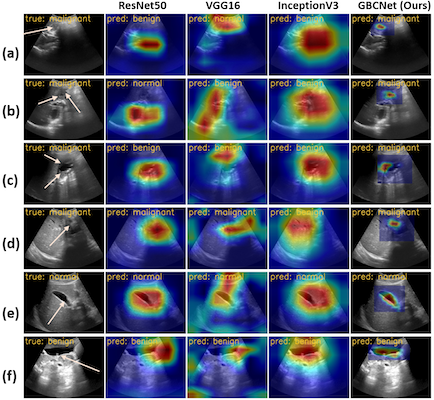
\includegraphics[width=0.62\linewidth]{figs/gbcnet/grad-cam.png}
	\caption[Qaualitative analysis of GBCNet with Grad-CAM visuals]{Grad-CAM visuals and the predictions for ResNet50, VGG16, Inception-V3, and GBCNet. The pathological areas are shown with arrows in the original images. 
	(a) ResNet50 and Inception-V3 focus on the shadow, whereas VGG16 focuses on the echogenic area, and all three fail to detect \gbc. GBCNet accurately focuses on the malignant \gb region invading the liver and detects \gbc.  (b), (c) The baseline networks focus on shadow or noise instead of the cancerous area and mispredict. 
	(d) Although ResNet50 and VGG16 predict malignancy, they fail to precisely focus on the malignant region compared to GBCNet. Inception-V3 failed to classify \gbc. (e), (f) GBCNet pinpoints the discriminating region compared to the baselines for normal and benign \gb regions, respectively. More visuals provided in \cref{fig:supple-2}.} %\ref{supp:cam_vis}.}
	\label{fig:gbc_vis}
\end{figure}

\begin{figure}[t]
	\centering
	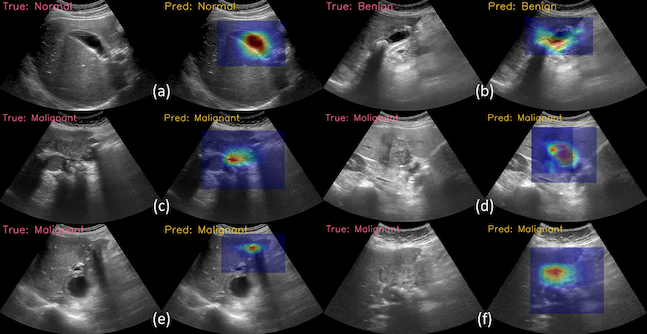
\includegraphics[width=0.7\linewidth]{figs/gbcnet/vis-s-1.png}
	\caption[Additional Grad-CAM visuals for GBCNet]{Sample Grad-CAM visuals of GBCNet with curriculum learning. (a) Normal, (b) Benign, and (c)--(f) Malignant samples.}
	\label{fig:supple-2}
\end{figure}

\section{Experiments and Results}
%
\subsection{Dataset}
%
We have used the image-based GBCU dataset described in \cref{chap:data} for the experiments. We recall that, there is a total of 1255 B-mode static abdominal USG images collected from 218 patients in this dataset. Each image is labeled as one of the three classes - normal, benign, or malignant, based on the biopsy reports. In addition to the classification labels, each image contains an axis-aligned bounding box spanning the entire \gb and adjacent liver parenchyma to annotate the \roi. The \roi in each image is drawn in consensus by two expert radiologists with 10 and 2 years of experience in abdominal radiology. The \roi (bounding box) annotations were used to train the \gb region selection network in the first stage of the GBCNet. The classification network in the second stage was trained using the image class labels. 

\mypara{Dataset Statistics}
%
Overall, we have 990 non-malignant (432 normal and 558 benign) and 265 malignant images. Of the 218 patients, 71, 100, and 47 belong to the normal, benign, and malignant classes, respectively. The width of the images was between 801 to 1556 pixels, and the height was between 564 to 947 pixels due to the cropping of patient-related information. 

\mypara{Dataset Splits}
%
The sizes of the training and testing sets are 1133 and 122, respectively. To ensure generalization to unseen patients, all images of any particular patient were either in the train or the test split. The number of normal, benign, and malignant samples in the train and test set is 401, 509, 223, and 31, 49, and 42, respectively. 
Since the dataset size is small, we also report the 10-fold cross-validation metrics on the entire dataset for key experiments to assess generalization. All images of any particular patient appeared either in the training or the validation split during the cross-validation. 

\subsection{Efficacy of GBCNet over Baselines}
%
We compare GBCNet with three popular deep classifiers, ResNet-50 \cite{resnet}, VGG-16 \cite{vgg}, and Inception-V3 \cite{inception}. We also evaluate the performance of three \sota object detectors, Faster-RCNN \cite{fasterrcnn}, RetinaNet \cite{retinanet}, and EfficientDet \cite{efficientdet} for detecting \gbc. We report the results in \cref{tbl:perf_gbc}. From the reported results, it is clear that baseline networks have poor accuracy for detecting \gbc from \usg images. Grad-CAM \cite{gradcam} visualizations in \cref{fig:gbc_vis} show that the noise, textures, and artifacts significantly influence the decision of baseline classification models. Additionally, \cref{fig:supple-2} shows the sample Grad-CAM visualizations of the predictions using GBCNet (ROI+MS-SoP) with curriculum learning. As highlighted in \cref{sec:usg_artifact_issue}, the standard DNN models tend to focus on the large shadow regions, and as a result, their classification accuracy suffers heavily. The shadow regions resembles the visual characteristics of a normal gallbladder (dark, anoechoic region). Compared to the baselines, GBCNet along-with the proposed MS-SoP classifier precisely focuses on crucial visual cues leading to its superior performance. 
%
\begin{table}[t]
	\centering
	\footnotesize
%	\captionsetup{width=\linewidth}
%    \setlength{\tabcolsep}{6pt}
%	\resizebox{\linewidth}{!}
	\caption[Comparison of the \gb region selection models]{Comparison of the \gb region selection models. We reported 10-fold cross validation (Mean$\pm$SD) of the metrics.}
\label{tbl:perf_region}
\end{table}
%
\begin{figure}[t]
	\centering
	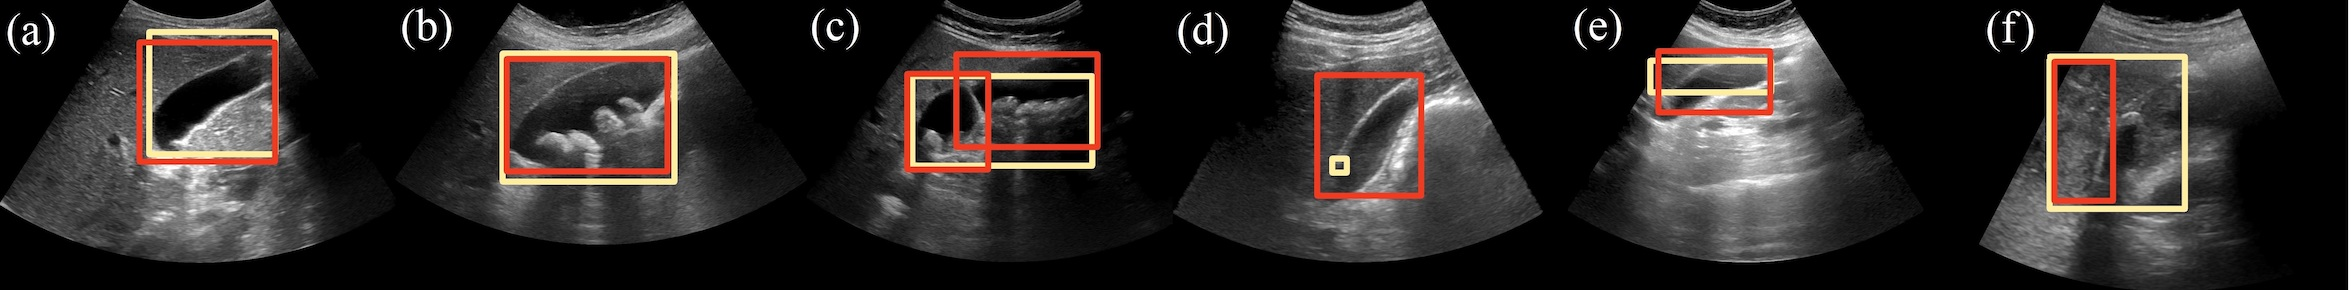
\includegraphics[width = \linewidth]{figs/roi_preds.jpg}%{figs/gbcnet/roi_preds.jpg}
	\caption[Comparison between the ROIs predicted by Faster-RCNN with radiologists]{We visually compare \roi selection by Faster-RCNN (dark red) with the \roi identified by expert Radiologists (light yellow). (a, b) The predicted a\roi matches well with the radiologists' expectations. (c) The model considers the sections partitioned by the \gb wall as separate regions. However, the union of the predicted boxes very closely approximates the actual \gb region. (d, e) Although the radiologist made an error in judging the \roi, Faster-RCNN was able to identify an accurate \roi resulting in a visually superior prediction. (f) The predicted \roi covers only a portion of the area an expert radiologist considered necessary. Even though the region prediction seems inferior compared to the human perception, expert radiologists corroborated that the predicted region captures the \gb invading the liver, a vital visual cue to detect \gbc. \roi samples from other detectors are in Appendix \cref{fig:supple-1}.}
	%\ref{supp:roi_vis}.}
	\label{fig:region_vis}
\end{figure}
%
\begin{figure}[t]
	\centering
	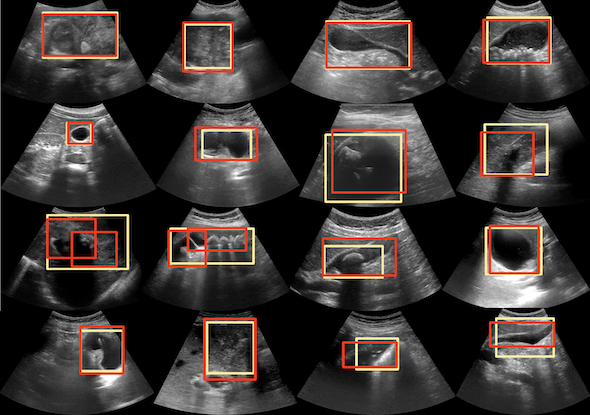
\includegraphics[width=0.7\linewidth]{figs/gbcnet/vis-s-0.png}
	\caption[Additional ROI visuals]{Sample visual results of RoI Detection models. First row - Faster-CNN, second row - YOLOv4, third row - Reppoints, and fourth row - CentripetalNet. Dark red is the ROI prediction by the model and light yellow is expert radiologists' perception of ROI.}
	\label{fig:supple-1}
\end{figure}
%
%\section{Appendix}
%
%
%\subsection{GradCAM Visuals for GBCNet}
%\label{supp:cam_vis}
Figure \ref{fig:supple-2} shows the sample Grad-CAM visualizations of the predictions using GBCNet (ROI+MS-SoP) with curriculum learning. %The blue regions show the most vital regions used by the classifier during prediction. The classifier well emphasized the crucial visual cues during inference.  

% \subsection{Candidate ROI Visuals}
% \label{supp:roi_vis}
% In figure \ref{fig:supple-1}, we show sample predictions of the GB region localization for different models. We also show the region of interest as perceived by the expert radiologists. The localization model is fairly accurate in capturing important regions of the USG image.

%
%
%\mypara{Performance of \gb Region Selection Models}
\subsection{Performance of GB Region Selection Models}
%
\cref{tbl:perf_region} summarizes the performance of various models for localizing the \gb region. For critical tasks such as region selection for cancer detection, recall is more important than precision. Multiple predicted regions can be discarded in the second stage, but missing any potentially malignant region could be disastrous. We note that the Faster-RCNN achieves the highest mIoU out of all the models while maintaining very high recall and excellent precision. Hence, we use Faster-RCNN as the region selection model. In \cref{fig:region_vis} we show the visual comparison of the \gb localization results of Faster-RCNN along with the \rois annotated by the expert radiologists. The model could predict the region of interest accurately in most cases. Although the model's prediction visually differed from the radiologists in some samples, closer inspection revealed that the predicted region retains sufficient visual cues to detect malignancy. In figure \ref{fig:supple-1}, we show additional sample predictions of the GB region localization for different models. 

\begin{table}[t]
	\centering
    \footnotesize
    \begin{tabular}{@{}lccc@{}}
    \toprule[1pt]
    \textbf{Model} & \textbf{Spec.} & \textbf{Sens.} \\
    \midrule[0.5pt]
    ResNet50 &  0.975 $\pm$ 0.024 & 0.829 $\pm$ 0.088\\
    DenseNet121  & 0.968 $\pm$ 0.018 & 0.824 $\pm$ 0.027 \\
    \midrule[0.5pt]
    MS-SoP (ours) & 0.967 $\pm$ 0.027 & 0.871 $\pm$ 0.071 \\
    \bottomrule[1pt]
    \end{tabular}
	\caption[Breast cancer detection results]{The sensitivity and specificity of MS-SoP and two baseline classifiers on breast cancer detection from USG images. We report 5-fold cross-validation on the BUSI dataset.}
\label{tbl:busi}
\end{table}

\begin{table}[t]
	\centering
	\footnotesize
	%\captionsetup{width=\linewidth}
    %\setlength{\tabcolsep}{10pt}
%    \resizebox{ \linewidth}{!}{%
    \begin{tabular}{lcccc}
    \toprule[1pt]
    \multirow{2}{*}{\textbf{Model}} & \multicolumn{2}{c}{\textbf{Orig. Test Set}} & \multicolumn{2}{c}{\textbf{Synth. Test Set}} \\
    & \textbf{Spec.} & \textbf{Sens.} & \textbf{Spec.} & \textbf{Sens.}\\
    \midrule[0.5pt]
    %AR+VGG16 & 51.6 & 56.3 & 88.1 & 55.7 ($\downarrow$) & 62.5 ($\downarrow$) & 88.1 \\
    ROI+VGG16 & 0.838 & 0.572 & 0.787 ($\downarrow$~~6.1\%) & 0.572 \\
    ROI+VGG16+VA & 0.825 & 0.762 & 0.775 ($\downarrow$~~6.1\%) & 0.762 \\
    \midrule
    %AR+ResNet50 & 84.3 & 85.7 & 88.6 & 71.3 ($\downarrow$) & 65.0 ($\downarrow$) & 88.6 \\
    %AR+ResNet50+curriculum & 91.8 & 93.8 & 97.6  & 88.5 ($\downarrow$) & 87.5 ($\downarrow$) & 97.6 \\
    ROI+ResNet50 & 0.863 & 0.857 & 0.650 ($\downarrow$24.7\%)& 0.857 \\
    ROI+ResNet50+VA & 0.938 & 0.857 & 0.887 ($\downarrow$~~5.4\%) & 0.857 \\
    \midrule
    ROI+Inception-V3 & 0.563 & 0.833 & 0.413 ($\downarrow$26.6\%) & 0.833 \\
    ROI+Inception-V3+VA & 0.913 & 0.690 & 0.788 ($\downarrow$13.7\%) & 0.690 \\
    \midrule
    GBCNet & 0.900 & 0.929 & 0.762 ($\downarrow$15.3\%) & 0.929 \\
    GBCNet+VA & 0.950 & 0.976 & 0.850 ($\downarrow$10.5\%) & 0.976 \\
    \bottomrule[1pt]
    \end{tabular}
%    }
    \caption[Robustness of the visual acuity curriculum in tacking texture bias]{Robustness of the curriculum in tacking texture bias while detecting \gbc. We show the performance of using curriculum on four models that apply classifiers on localized \gb region - (a) ROI+VGG16, (b) ROI+ResNet50, (c) ROI+Inception-V3, and (d) GBCNet (ROI+MS-SoP). The relative change (in percentage) in specificity for synthetic test data is shown within parentheses. The sensitivity remains unchanged as the malignant images were not altered. Observe that as compared to the models trained on high-resolution images, our VA-based curriculum is more robust to textures and is able to maintain a lower drop in specificity. The only exception is the ROI+VGG16 model, for which the curriculum training does not lower the drop in specificity. }
    %Also, note how the proposed curriculum is able to improve the performance of all four networks.}
\label{tbl:curr_texture}
\end{table}

\subsection{Applicability of the Proposed Classifier in Breast Cancer Detection from USG Images}
%
We explored the applicability of the proposed MS-SoP classifier on breast cancer detection from \usg images for a publicly available dataset, BUSI \cite{al2020dataset}, containing 133 normal, 487 benign, and 210 malignant images. The images in BUSI are already cropped from original \usg images to highlight only the important regions. Thus, we skip the \roi selection and run the MS-SoP classifier on BUSI. \cref{tbl:busi} shows that the MS-SoP classifier achieves much better sensitivity, which indicates the superiority of the MS-SoP architecture for malignancy identification on \usg images. We note that while breast cancer detection relies on tissue/ mass characterization, \gbc detection is primarily based on wall shape and mass anomaly. %The performance gain using MS-SoP on these two different types of cancers is interesting to note.
\par We remark that, while the MS-SoP classification network was applicable on both tasks, the Visual Acuity-based curriculum may not be suitable for Breast Cancer Detection. Breast cancer detection from USG relies heavily on the textures of the mass/ tissue in the images, as opposed to the wall shape and mass forming anomalies in GBC. Thus, while using a smoothing-based curriculum to bias the learning towards shape features is conducive for GBC detection, it may not aid breast cancer detection.

\begin{figure}[t]
	\centering
	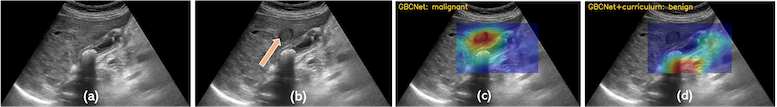
\includegraphics[width=0.9\linewidth]{figs/gbcnet/texture_vis_curr.png}
	\caption[Visualization of the effect of curriculum]{(a) Original image of a benign \gb. The \gb presents a stone and thickened wall. (b) In the synthetic image, we added an artificial tissue-like patch near the benign \gb region (highlighted by the arrow). This patch is not a part of the original \gb, and expert radiologists confirmed that the diagnosis of the \gb is not altered. (c) The textured artificial patch makes the GBCNet biased, and it focuses on the patch to predict the sample as malignant (false-positive). (d) Visual acuity curriculum fixes the texture bias of the GBCNet and helps the network to re-adjust the salient regions to the actual \gb pathology. %and learn the visual cues of a non-malignant \gb such as stone or a thickened wall.
}
	\label{fig:texture_vis}
\end{figure}

\subsection{Efficacy of the Proposed Curriculum}
%
\myfirstpara{Robustness in Tackling Texture Bias}
As described earlier, spurious textures present in \usg images tend to increase the false positives in detecting malignancy. To validate this hypothesis, we created a synthetic test set. We used the method given by \cite{yang2020fda} and added low-level frequencies from malignant images to alter the original texture of normal and benign samples. We also manually added patches looking like soft tissue near the \gb region of normal and benign images. Expert radiologists confirmed that the diagnosis of the \gb pathology is not altered. \cref{tbl:curr_texture} shows that the specificity decreases due to the increase of the false positives. The sensitivity remains unaffected as the prediction for malignant \gb samples was unchanged. The network trained with the proposed curriculum tackles texture bias well and accurately predicts non-malignant samples in synthetic test data. This experiment shows that the proposed curriculum effectively tackles texture bias. \cref{fig:texture_vis} shows a visual sample of how the soft tissue-like texture influences the network's decision and how the curriculum helps the network to rectify the discriminative regions. 

\begin{table}[t]
	\centering
	\footnotesize
%	\captionsetup{width=\linewidth}
%    \setlength{\tabcolsep}{6pt}
%	\resizebox{\linewidth}{!}{%
    \begin{tabular}{@{}lccc@{}}
    \toprule[1pt]
    \textbf{Model} & \textbf{Acc} & \textbf{Spec.} & \textbf{Sens.} \\
    \midrule[0.5pt]
    ROI+VGG16 & 0.533 $\pm$ 0.092 & 0.719 $\pm$ 0.115 & 0.733 $\pm$ 0.179\\
    ROI+VGG16+VA & 0.777 $\pm$ 0.041 & 0.938 $\pm$ 0.030 & 72.0 $\pm$ 0.195\\
    \midrule
    ROI+ResNet50 & 0.766 $\pm$ 0.107 &  0.823 $\pm$ 0.105 & 0.909 $\pm$ 0.111\\
    ROI+ResNet50+VA & 0.854 $\pm$ 0.077 & 0.923 $\pm$ 0.059 & 0.875 $\pm$ 0.091 \\
    \midrule
    ROI+Inception-V3 & 0.718 $\pm$ 0.089 & 0.833 $\pm$ 0.087 & 0.785 $\pm$ 0.214\\
    ROI+Inception-V3+VA & 0.826 $\pm$ 0.046 & 0.931 $\pm$ 0.044 & 0.826 $\pm$ 0.099\\
    \midrule
    % RetinaNet & 74.9 $\pm$ 7.3 &  86.7 $\pm$ 7.8 & 79.1 $\pm$ 8.9\\
    % RetinaNet+VA & 73.3 $\pm$ 6.0 & 92.1 $\pm$ 4.4 & 70.6 $\pm$ 14.2\\
    % \midrule
    GBCNet (ROI+MS-SoP) & 0.882 $\pm$ 0.051 & 0.942 $\pm$ 0.037 & 0.923 $\pm$ 0.071\\
    GBCNet+VA & 0.921 $\pm$ 0.029 &  0.967 $\pm$ 0.023 & 0.919 $\pm$ 0.063\\
    \bottomrule[1pt]
    \end{tabular}
%	}
	\caption[Model performances for training with visual acuity curriculum]{Model performances (10-fold cross-validation) for training with our proposed visual acuity-based curriculum.}
\label{tbl:curr_improve}
\end{table}

\mypara{Performance Improvement with Proposed Curriculum}
We also assess the quantitative performance improvement of models due to the curriculum training in \cref{tbl:curr_improve}. All models show improvement in specificity, which indicates the effectiveness of the proposed blurring-based curriculum in tackling texture bias, and reducing false positives. 

%\subsubsection{Generalization to multiple resolutions}
%%
%To verify how well can the curriculum enhance the generalization capability of \GBCNet at different resolutions, we evaluate the performance of the \GBCNet on the test set at different resolutions. We do this by blurring the test set using different values of $\sigma$ and evaluating GBCNet on these images. Like before, we evaluated the GBCNet without any curriculum and GBCNet with curriculum, anti-curriculum, and the control-curriculum models. The results of this comparison can be seen in \cref{fig:gbc_curr_blur}. The model trained using our proposed curriculum generalizes well across a larger spectrum of image resolutions, and this is an indicator of better spatial understanding than the other models. Note that, the blurred images improve the detection of non-malignant test samples (\cref{fig:spec-test-blur}) for all models. This is an alternate validation of the hypothesis that non-malignant samples (normal and benign) learn better from shape than textures. An interesting observation is that the anti-curriculum performs well at highly blurred (low-resolution) test samples. This can be explained from the fact that anti-curriculum is presented with low-resolution images towards the end of the training cycle. Thus, it maintains the sensitivity better for low-resolution test samples. The curriculum-based GBCNet learns high resolution images towards the later part of the training and thus the sensitivity starts to degrade with low resolution images.

\begin{figure}[t]
	\centering
	\begin{subfigure}[b]{0.23\linewidth}
    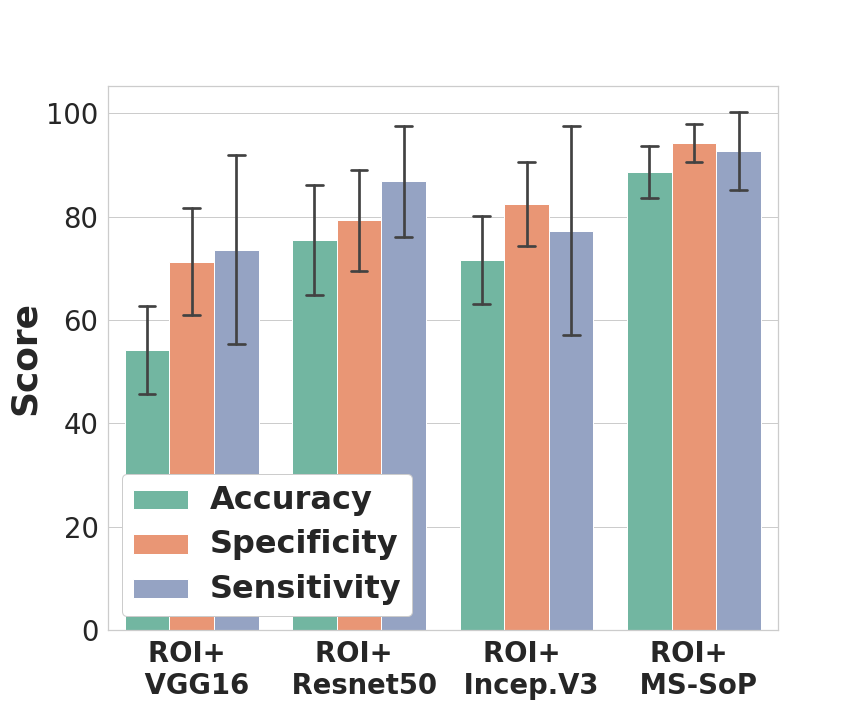
\includegraphics[width=\linewidth]{figs/gbcnet/roi_models.png}
    \caption{}
    \label{fig:perf_attn_models}
    \end{subfigure}
	\begin{subfigure}[b]{0.23\linewidth}
		\centering
		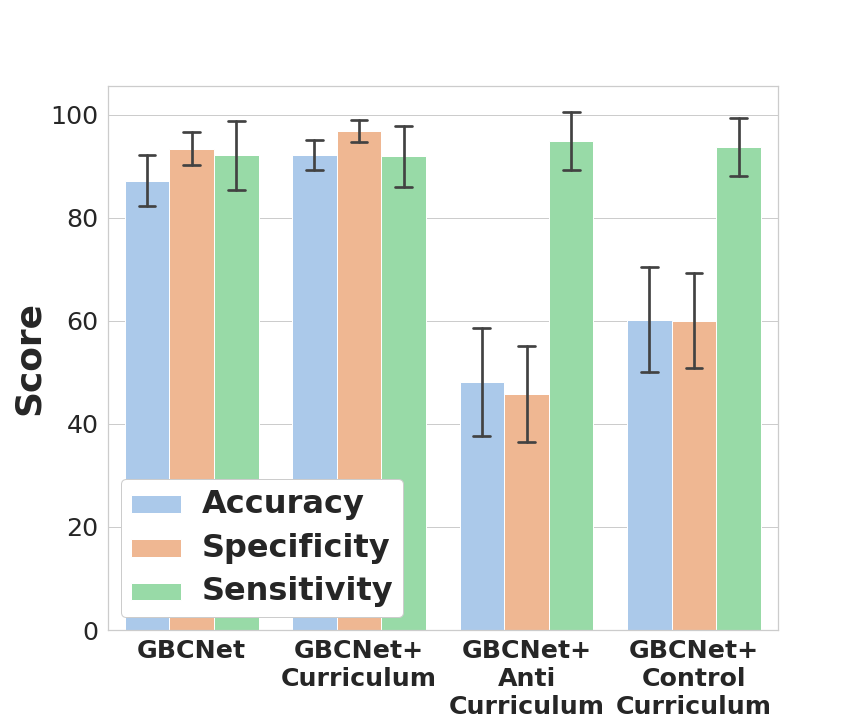
\includegraphics[width=\linewidth]{figs/gbcnet/curr_pred.png}
		\caption{}
		\label{fig:ablation1}
	\end{subfigure}
	%
	\begin{subfigure}[b]{0.23\linewidth}
		\centering
		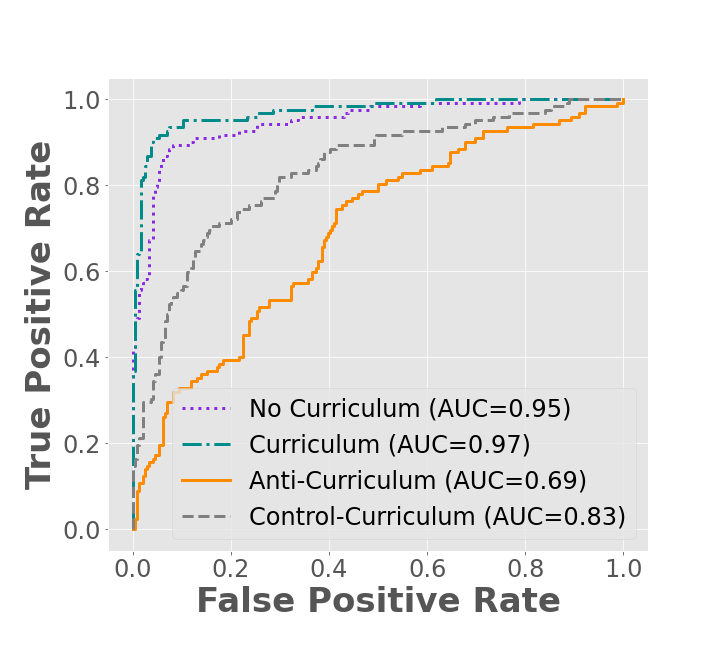
\includegraphics[width=\linewidth]{figs/gbcnet/roc.png}
		\caption{}
		\label{fig:ablation2}
	\end{subfigure}
		\begin{subfigure}[b]{0.23\linewidth}
		\centering
		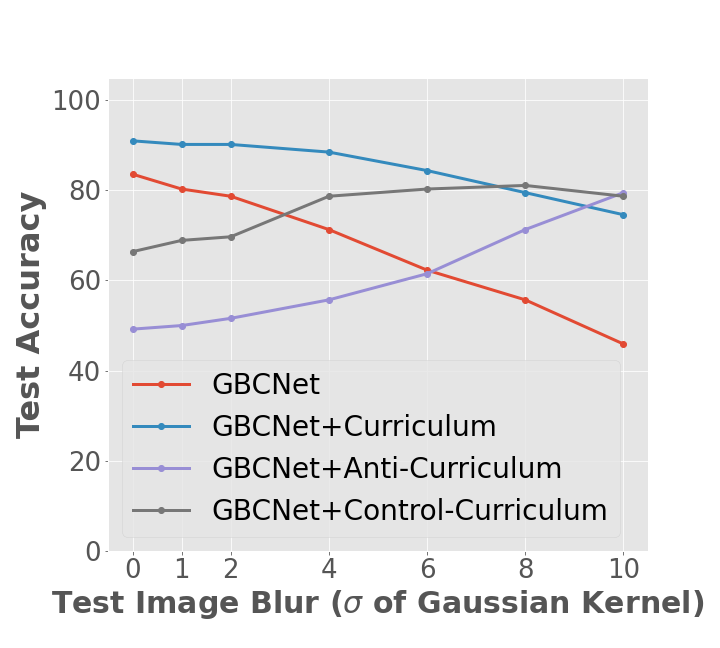
\includegraphics[width=\linewidth]{figs/gbcnet/acc-mr.png}
		\caption{}
		\label{fig:ablation3}
	\end{subfigure}
	\caption[Ablation study]{Ablation study. (a) Comparison of accuracy, specificity, and sensitivity for applying different classification networks (VGG16, ResNet50, Inception-V3, and MS-SoP) on the localized \gb. We have reported the 10-fold cross validation results. (b) The efficacy of the proposed training regime in terms of accuracy, specificity, sensitivity. (c) ROC-AUC for different training regimes on the test set. (d) The proposed curriculum generalizes better at different resolutions. }
	\label{fig:diff_images}
\end{figure}

\subsection{Ablation Study}
%
\myfirstpara{Choice of Classifier in GBCNet}
%
We have plugged in other deep classification networks in place of the proposed MS-SoP classifier in the GBCNet framework. \cref{fig:perf_attn_models} summarizes the results. The MS-SoP classifier on GBCNet provides the best \gbc detection accuracy. Using the classifiers on the \rois improves the sensitivity and accuracy for ResNet50 and VGG16. However, the drop in specificity results in performance degradation for Inception-V3 as the sensitivity was not improved.  

\mypara{Choice of Training Regime}
%
We used the proposed GBCNet model to assess the influence of the visual acuity-based curriculum. We compare the curriculum with two possible alternatives - (i) \emph{anti-curriculum} that initially trains with high resolution and progressively lowers the resolution, and (ii) \emph{control-curriculum} where the samples are not sorted resolution-wise, and the curriculum contains a random set of blurred samples. Note that the control-curriculum can also be thought of using Gaussian blurring as a data augmentation where the probability of choosing a particular $\sigma$ is equal to the fraction of epochs the $\sigma$ used during the curriculum. \cref{fig:ablation1} and \ref{fig:ablation2} show the performance of the various curriculum strategies on the performance on GBCNet.  %\cref{fig:gbc_curr_blur} shows the ROC with the AUC for GBCNet with different curriculum. 
%Additionally, \cref{tbl:curr_texture} shows the performance improvement of attention region-based classifiers when trained with the proposed curriculum.
Further, to understand how various curriculum strategies affect a model's generalization at different resolutions, we blur the test set using different values of $\sigma$ and evaluate the models on these images (\cref{fig:ablation3}). 
%The results of this comparison can be seen in \cref{fig:ablation3}. 
We see that the model trained using the proposed curriculum generalizes well across different image resolutions, which is an indicator of better spatial understanding.

\begin{table}[t]
	\centering
	\footnotesize
%	\captionsetup{width=\linewidth}
%    \setlength{\tabcolsep}{6pt}
%	\resizebox{\linewidth}{!}{%
    \begin{tabular}{@{}lccc@{}}
    \toprule[1pt]
    \textbf{Model} & \textbf{Spec.} & \textbf{Sens.} \\
    \midrule[0.5pt]
    ROI+MS-SoP (GBCNet) & 0.942 $\pm$ 0.037 & 0.923 $\pm$ 0.071 \\
    ROI+MS-SoP (channel-wise pooling) & 0.904 $\pm$ 0.047 & 0.861 $\pm$ 0.068  \\
    ROI+MS-SoP (spatial pooling) & 0.900 $\pm$ 0.064 & 0.882 $\pm$ 0.064 \\
    ROI+MS (w/o SoP) & 0.887 $\pm$ 0.060 & 0.872 $\pm$ 0.064 \\
    ROI+SoP (w/o MS) & 0.914 $\pm$ 0.048 & 0.854 $\pm$ 0.079 \\
    \bottomrule[1pt]
    \end{tabular}
%	}
	\caption[Ablation of the proposed MS-SoP network]{Ablation of Ms-SoP. We show the specificity and sensitivity of MS-SoP with two alternatives - MS-SoP with (i) only channel-wise and (ii) only spatial pooling. We also show the efficacy of using multi-scale and second-order pooling in conjunction.}
\label{tbl:ms-sop-ablation}
\end{table}

\mypara{Components of the MS-SoP Classifier}
%
We present the ablation study on the MS-SoP classifier in \cref{tbl:ms-sop-ablation}. We show the effect of the multi-scale and second-order pooling components on the specificity and sensitivity of the model. We also show the relevance of the channel-wise and spatial pooling in the second-order pooling.
\section{Conclusion}
%\todo{We have observed that our proposed system fails to capture the inaccuracies caused by the small mass or irregular structures near the gallbladder wall. Since gallbladder is a hollow organ, the malignancy starts from the wall. For nearly 5\% of the images, the irregularity and minuscule structures of the wall needs discerning between the noise, soft tissue texture, and the tiny wall structure.} 
In this chapter, we addressed Gallbladder Cancer detection from USG images using deep learning and proposed a new supervised learning framework (GBCNet) based on \roi selection and a multi-scale second-order pooling. The proposed design helps the classifier focus on the crucial \gb region predicted by the region selection network, and make better predictions by mitigating the effect of noise and artifacts. We also tested the performance of the proposed MS-SoP classifier on breast cancer detection from USG. The performance gain using MS-SoP on these two different types of cancers indicates that the model is capable of learning robust representations of different types of malignancy in USG images. We also proposed a visual acuity-based curriculum to make our design resilient to texture bias and improve its specificity of GBCNet. Extensive experiments show that GBCNet, combined with the curriculum learning, improves performance over the baseline deep classification and object detection architectures. Our work tackles the impediments posed by \usg images towards making accurate GBC detection, an important but hitherto overlooked problem.
%In the future, we would like to explore if the proposed network architecture and the visual acuity-based curriculum can help improve predictions in other cancer detection problems.
%We chose breast cancer detection, a prominent problem in this domain, and validated the MS-SoP classifier on the public breast ultrasound image (BUSI) dataset. We note that while breast cancer detection relies on tissue/ mass characterization, GBC detection is primarily based on wall shape and mass anomaly. The performance gain using MS-SoP on these two different types of cancers indicates efficient malignancy representation by our model. We plan to evaluate our method on other datasets as future work to formally understand the efficacy and the characterization of malignancy representation by MS-SoP for different types of cancers.

%{\small \mypara{Acknowledgement} The authors thank IIT Delhi HPC facility for computational resources.}
%\begin{figure}[t]
	\centering
	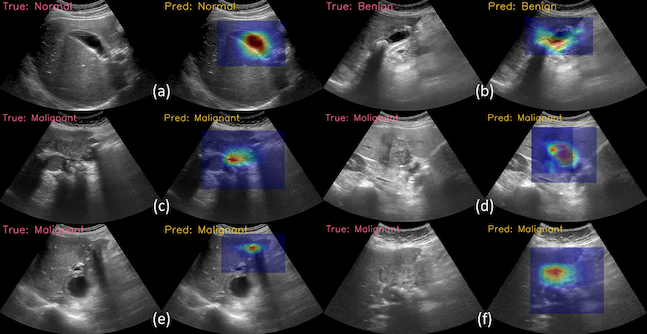
\includegraphics[width=0.7\linewidth]{figs/gbcnet/vis-s-1.png}
	\caption[Additional Grad-CAM visuals for GBCNet]{Sample Grad-CAM visuals of GBCNet with curriculum learning. (a) Normal, (b) Benign, and (c)--(f) Malignant samples.}
	\label{fig:supple-2}
\end{figure}

\begin{figure}[t]
	\centering
	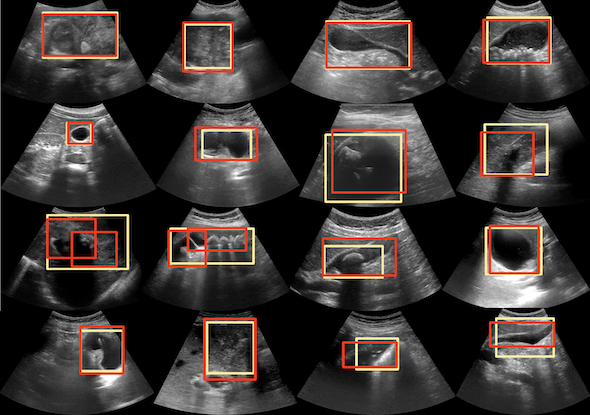
\includegraphics[width=0.7\linewidth]{figs/gbcnet/vis-s-0.png}
	\caption[Additional ROI visuals]{Sample visual results of RoI Detection models. First row - Faster-CNN, second row - YOLOv4, third row - Reppoints, and fourth row - CentripetalNet. Dark red is the ROI prediction by the model and light yellow is expert radiologists' perception of ROI.}
	\label{fig:supple-1}
\end{figure}

\section{Appendix}


\subsection{GradCAM Visuals for GBCNet}
\label{supp:cam_vis}
Figure \ref{fig:supple-2} shows the sample Grad-CAM visualizations of the predictions using GBCNet (ROI+MS-SoP) with curriculum learning. %The blue regions show the most vital regions used by the classifier during prediction. The classifier well emphasized the crucial visual cues during inference.  

\subsection{Candidate ROI Visuals}
\label{supp:roi_vis}
In figure \ref{fig:supple-1}, we show sample predictions of the GB region localization for different models. We also show the region of interest as perceived by the expert radiologists. The localization model is fairly accurate in capturing important regions of the USG image.

\subsection{Baseline Implementation Details}
%

\label{supp:impl}
\cref{tbl:configs} lists the configurations of all models which we have used. We trained on the Quadro P5000 16GB GPU. The table includes a brief description of the various stages of the network, input image sizes ($H\times W\times D$), the optimizer, relevant hyper-parameters such as learning rate, weight decay, momentum, batch size, and the number of training epochs/steps for the network. 
 \begin{table}[t]
\centering
\footnotesize
%\setlength{\tabcolsep}{4pt}
    \resizebox{ \linewidth}{!}{%
        \begin{tabular}{p{0.1\linewidth}p{0.42\linewidth}p{0.06\linewidth}p{0.2\linewidth}p{0.05\linewidth}p{0.06\linewidth}}
        \toprule[1.5pt]
        \textbf{Model} & \textbf{Description} & \textbf{Input Size} & \textbf{Optimizer} & \textbf{Batch size} & \textbf{Epochs/ Steps}
        \\ \midrule[0.75pt]
        YOLOv4 \cite{yolov4} & CSPDarknet53 backbone, PANet neck, anchor-based YOLO head. Total 162-layers. Backbone was frozen for first 800 step. Entire network was trainable thereafter. Single stage, anchor-based  & $608\times608\times3$ & SGD LR = 0.0001 momentum = 0.95 weight decay = 0.0005 & 64 & 3000 steps \\ \hline
        Reppoints \cite{reppoints} & Resnet-101 backbone, Group Normalization neck, and a reppoints head. Backbone was frozen for first 30 epochs, and entire network was trainable thereafter. Two-stage, anchor-free & $800 \times 1333 \times 3$ & SGD LR = 0.001 momentum = 0.9 weight decay = 0.0001 & 4 & 50 epochs \\ \hline
        Centripetal-Net \cite{centripetalnet} & HourglassNet-104 backbone. Enitre network was trainable. Anchor-free & $511 \times 511 \times 3$ & Adam LR = 0.0005 & 4 & 50 epochs \\ \hline
        ResNet \cite{resnet} & Resnet-50 used. All layers were trainable. LR decays by 10\% after every 5 epochs through a step LR scheduler. & $224\times224\times3$ & SGD LR = 0.005 momentum = 0.9 weight decay = 0.0005 & 16 & 100 epochs \\ \hline
        VGG \cite{vgg} & VGG-16 is used. All layers were trainable. LR decays by 10\% after every 5 epochs through a step LR scheduler. & $224\times224\times3$ & SGD LR = 0.005 momentum = 0.9 weight decay = 0.0005 & 16 & 100 epochs \\ \hline
        Inception \cite{inception} & Inception-V3 used. All layers were trainable. LR decays by 10\% after every 5 epochs through a step LR scheduler. & $299\times299\times3$ & SGD LR = 0.005 momentum = 0.9 weight decay = 0.0005 & 16 & 100 epochs \\ \hline
        RetinaNet \cite{retinanet} & Resnet-18-FPN used as backbone. All layers were trainable. & $512\times512\times3$ & Adam LR = 0.0001 & 8 & 50 epochs \\ \hline
        EfficientDet \cite{efficientdet} & EfficientNet-B4 used as backbone and BiFPN as feature network. All layers were trainable. & $1024\times1024\times3$ & Adam LR = 0.001 & 2 & 50 epochs \\ 
        \bottomrule
    \end{tabular}
    }
    \caption[Implementation details for the different baseline networks]{Implementation details for the different baseline networks used for classification and \gb localization.}
    \label{tbl:configs}
\end{table}






